% Copyright (c) 2026 JoltWare
% SPDX-License-Identifier: Apache-2.0

\documentclass[11pt,a4paper,openany]{report}

\usepackage[T1]{fontenc}
\usepackage[utf8]{inputenc}
\usepackage{lmodern}
\usepackage[margin=2.4cm]{geometry}
\usepackage{graphicx}
\usepackage{xcolor}
\usepackage{booktabs}
\usepackage{tabularx}
\usepackage{longtable}
\usepackage{enumitem}
\usepackage{listings}
\usepackage{caption}
\usepackage{float}
\usepackage{titlesec}
\usepackage{fancyhdr}
\usepackage[most]{tcolorbox}
\usepackage{tikz}
% Code must print as typed: without this, the T1 typewriter font turns -- into a dash, << >> into
% guillemets and `` into a quote. Only ligatures are touched (protrusion and expansion stay off).
\usepackage[protrusion=false,expansion=false]{microtype}
\DisableLigatures[-,<,>,`,']{encoding = T1, family = tt*}
\usetikzlibrary{arrows.meta,positioning,fit,calc,backgrounds,shapes.multipart,shapes.geometric}
\usepackage[colorlinks=true,linkcolor=accent,urlcolor=accent]{hyperref}

\definecolor{accent}{HTML}{2B4C8C}
\definecolor{codebg}{HTML}{F5F6FA}
\definecolor{gold}{HTML}{C8902E}
\definecolor{tipbg}{HTML}{EAF4EA}
\definecolor{tipframe}{HTML}{3A7D44}
\definecolor{notebg}{HTML}{EAF0FA}
\definecolor{warnbg}{HTML}{FBEFE3}
\definecolor{warnframe}{HTML}{C0661A}

\graphicspath{{images/}}
\setlength{\parskip}{0.45em}
\setlength{\parindent}{0pt}

\titleformat{\chapter}[display]{\normalfont\bfseries\color{accent}}{\large\chaptertitlename\ \thechapter}{0.4em}{\Huge}
\titlespacing*{\chapter}{0pt}{-10pt}{18pt}
\titleformat{\part}[display]{\centering\normalfont\bfseries\color{accent}}{\LARGE\partname\ \thepart}{1em}{\Huge}

\pagestyle{fancy}
\fancyhf{}
\fancyhead[L]{\small\color{black!60}MachinaState User Manual}
\fancyhead[R]{\small\color{black!60}\leftmark}
\fancyfoot[C]{\thepage}
\renewcommand{\headrulewidth}{0.3pt}
\renewcommand{\chaptermark}[1]{\markboth{\thechapter.\ #1}{}}
\setlength{\emergencystretch}{3em}

\lstdefinestyle{base}{
  basicstyle=\ttfamily\footnotesize,
  backgroundcolor=\color{codebg},
  frame=single,
  rulecolor=\color{black!15},
  keywordstyle=\color{accent}\bfseries,
  commentstyle=\color{black!55}\itshape,
  stringstyle=\color{gold!80!black},
  showstringspaces=false,
  breaklines=true,
  columns=fullflexible,
  keepspaces=true,
  xleftmargin=4pt,
  xrightmargin=4pt,
  numberstyle=\tiny\color{black!40}
}
\lstset{style=base}
\lstdefinelanguage{json}{
  morestring=[b]",
  comment=[l]{//},
  literate={:}{{\textcolor{accent}{:}}}1
}
\lstdefinestyle{output}{style=base, backgroundcolor=\color{black!3}, basicstyle=\ttfamily\scriptsize}

\newtcolorbox{tip}{colback=tipbg,colframe=tipframe,boxrule=0.4pt,arc=2pt,left=6pt,right=6pt,top=4pt,bottom=4pt,fonttitle=\bfseries\small,title=Tip}
\newtcolorbox{note}{colback=notebg,colframe=accent,boxrule=0.4pt,arc=2pt,left=6pt,right=6pt,top=4pt,bottom=4pt,fonttitle=\bfseries\small,title=Note}
\newtcolorbox{caution}{colback=warnbg,colframe=warnframe,boxrule=0.4pt,arc=2pt,left=6pt,right=6pt,top=4pt,bottom=4pt,fonttitle=\bfseries\small,title=Caution}

\newcommand{\ui}[1]{\textsf{\textbf{#1}}}
\newcommand{\code}[1]{\texttt{#1}}
\newcommand{\key}[1]{\tikz[baseline=(k.base)]\node[draw,rounded corners=2pt,inner sep=2pt,fill=black!4,font=\ttfamily\footnotesize](k){#1};}
\DeclareRobustCommand{\co}[1]{\tikz[baseline=(c.base)]\node[callout](c){#1};}

\newcommand{\screenshot}[3][0.92\linewidth]{%
  \begin{figure}[H]
    \centering
    \fbox{\includegraphics[width=#1]{#2}}
    \caption{#3}
    \label{fig:#2}
  \end{figure}}

\tikzset{
  st/.style={draw, rounded corners=6pt, minimum width=2.2cm, minimum height=0.95cm, fill=white, align=center, font=\small},
  composite/.style={draw, rounded corners=10pt, fill=accent!5, inner sep=10pt},
  init/.style={circle, fill=black, inner sep=0pt, minimum size=8pt},
  final/.style={circle, draw, thick, inner sep=0pt, minimum size=12pt, path picture={\fill (path picture bounding box.center) circle (3.2pt);}},
  hist/.style={circle, draw, thick, fill=white, inner sep=1pt, minimum size=16pt, font=\scriptsize\bfseries},
  choicept/.style={diamond, draw, thick, fill=white, inner sep=0pt, minimum size=16pt},
  tr/.style={-{Stealth[length=7pt]}, thick},
  lbl/.style={font=\scriptsize\ttfamily, fill=white, inner sep=1.5pt},
  callout/.style={circle, fill=gold, text=white, font=\bfseries\footnotesize, inner sep=1.2pt, minimum size=15pt, draw=white, line width=0.8pt},
  stepno/.style={circle, fill=accent, text=white, font=\bfseries\scriptsize, inner sep=1pt, minimum size=12pt},
  box/.style={draw, rounded corners=3pt, fill=white, align=center, font=\small, minimum height=1cm, inner sep=5pt}
}

\begin{document}

\pagenumbering{Alph}
%=====================================================================
\begin{titlepage}
  \centering
  \vspace*{2cm}
  
\includegraphics[width=4.5cm]{../media/MachinaState.png}\par\vspace{1.2cm}
  {\Huge\bfseries\color{accent} MachinaState\par}\vspace{0.4cm}
  {\Large Visual UML State Machine Designer for Visual Studio Code\par}\vspace{0.3cm}
  {\large User Manual\par}\vspace{1.5cm}
  \begin{minipage}{0.8\linewidth}\centering
    Draw, simulate and generate hierarchical state machines\\
    in C++, C\# and C --- switch-based or table-based.
  \end{minipage}\par
  \vfill
  {\large Version 1.0.0 \quad\textbullet\quad \today\par}
\end{titlepage}

\pagenumbering{roman}
\tableofcontents
\cleardoublepage
\pagenumbering{arabic}

%=====================================================================
\part{Getting Started}

\chapter{Introduction}

\section{What is MachinaState?}
MachinaState is a Visual Studio Code extension for designing \emph{state machines} visually and turning
them into production code. You draw a UML state machine diagram on a canvas, check its behaviour in a
built-in simulator, and generate a C++ or C\# class, or a C module, that implements it. Your own logic
--- what happens when a light switches on or a door unlocks --- lives in a hand-written subclass (in C,
in functions you register), so the diagram can be changed and regenerated at any time without
touching your code.

A state machine describes a system that is always in one of a finite number of \emph{states} (with
orthogonal regions, in one state per region) and moves between them in response to \emph{events}. Typical examples are protocol handlers, user
interface flows, device controllers, game characters and workflow engines. Writing such logic by hand
quickly leads to deeply nested \code{if} statements and flags; a diagram makes the behaviour explicit,
reviewable and testable.

\section{Feature overview}
\begin{itemize}[itemsep=1pt]
  \item \textbf{Visual editor}:
        \begin{itemize}[itemsep=0pt]
          \item states, composite (nested) states, initial and final states
          \item orthogonal (parallel) regions
          \item history pseudostates and choice points
          \item transitions with events, guards and actions; internal transitions, completion
                transitions and \code{after(...)} timeouts
          \item colours
        \end{itemize}
  \item \textbf{Productive editing}:
        \begin{itemize}[itemsep=0pt]
          \item multi-selection, align and distribute
          \item copy, cut, paste and duplicate (also between diagrams)
          \item arrow-key nudging and snap to grid
          \item automatic layout with the Eclipse Layout Kernel
        \end{itemize}
  \item \textbf{Continuous validation} in the editor and in VS Code's \ui{Problems} panel.
  \item \textbf{Interactive simulator} running the same reference engine that the test suite checks
        against the generated code:
        \begin{itemize}[itemsep=0pt]
          \item highlights the active states and records a trace of every exit, action and entry
          \item guard results as check boxes, event arguments and running timers
          \item scenarios that are recorded, saved in the diagram and replayed
          \item transition coverage
        \end{itemize}
  \item \textbf{Code generation}:
        \begin{itemize}[itemsep=0pt]
          \item C++ (C++17, single header, no heap allocation), C\# (C\# 8+) and C (C99, a header
                and a source file, no heap allocation)
          \item each as a \emph{switch-based} or \emph{table-based} implementation; all six variants
                behave identically and are verified against each other by an automated test suite
          \item optional regeneration on every save
        \end{itemize}
  \item \textbf{Hierarchical semantics}:
        \begin{itemize}[itemsep=0pt]
          \item event bubbling from inner to outer states
          \item exit/entry ordering via the least common ancestor
          \item default entry and shallow/deep history
          \item run-to-completion processing including completion transitions
        \end{itemize}
  \item \textbf{Event parameters} passed to guards and actions.
  \item \textbf{Options}:
        \begin{itemize}[itemsep=0pt]
          \item a tracing hook
          \item thread safety through user-implemented \code{Lock}/\code{Unlock} functions
          \item an \textbf{event queue} so that actions can raise follow-up events
          \item \textbf{timer hooks} for timeouts
        \end{itemize}
  \item \textbf{PlantUML, Mermaid and SCXML} import and export; \textbf{Copy as Mermaid} for Markdown documentation.
  \item \textbf{PNG and SVG export} and a diff-friendly JSON file format.
\end{itemize}

\section{How it works}
Figure~\ref{fig:pipeline} shows the workflow. The diagram is stored in a \code{.machina} file. The
generator turns it into an abstract class that contains the complete state handling. You derive from
that class and implement the \emph{hooks} --- guards, actions and optionally tracing and locking.

\begin{figure}[H]
\centering
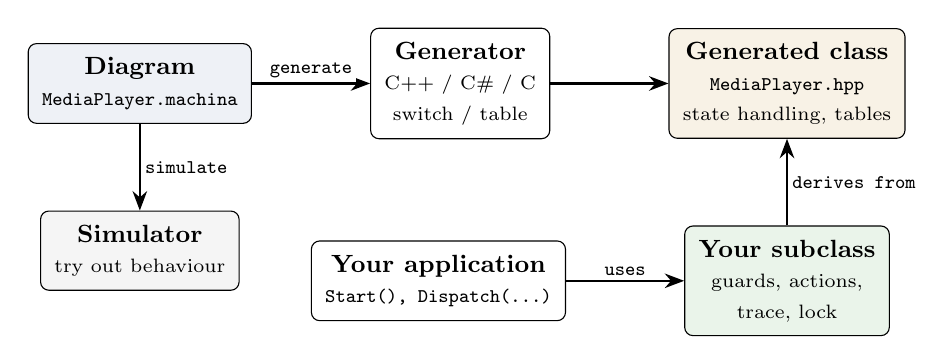
\begin{tikzpicture}[node distance=1.1cm and 1.5cm]
  \node[box, fill=accent!8] (diagram) {\textbf{Diagram}\\\scriptsize\ttfamily MediaPlayer.machina};
  \node[box, right=of diagram] (gen) {\textbf{Generator}\\\scriptsize C++ / C\# / C\\\scriptsize switch / table};
  \node[box, right=of gen, fill=gold!12] (cls) {\textbf{Generated class}\\\scriptsize\ttfamily MediaPlayer.hpp\\\scriptsize state handling, tables};
  \node[box, below=of cls, fill=tipbg] (user) {\textbf{Your subclass}\\\scriptsize guards, actions,\\\scriptsize trace, lock};
  \node[box, left=of user] (app) {\textbf{Your application}\\\scriptsize \ttfamily Start(), Dispatch(...)};
  \node[box, below=of diagram, fill=black!4] (sim) {\textbf{Simulator}\\\scriptsize try out behaviour};
  \draw[tr] (diagram) -- node[lbl, above]{generate} (gen);
  \draw[tr] (gen) -- (cls);
  \draw[tr] (user) -- node[lbl, right]{derives from} (cls);
  \draw[tr] (app) -- node[lbl, above]{uses} (user);
  \draw[tr] (diagram) -- node[lbl, right]{simulate} (sim);
\end{tikzpicture}
\caption{From diagram to running code.}
\label{fig:pipeline}
\end{figure}

\section{How to read this manual}
\begin{itemize}[itemsep=1pt]
  \item \textbf{Part~I} installs the extension and gives a guided tour of the editor.
  \item \textbf{Part~II} contains five hands-on tutorials that build complete, compiling examples:
        \begin{itemize}[itemsep=0pt]
          \item a simple traffic light (C++, switch-based)
          \item a hierarchical traffic light with fault handling and history (C++, table-based with
                tracing)
          \item a thread-safe door lock with event parameters (C\#, table-based)
          \item a vending machine with choice points, completion transitions, timeouts and the event
                queue (C++, switch-based)
          \item a washing machine with orthogonal regions, recorded scenarios and coverage (C\#)
        \end{itemize}
  \item \textbf{Part~III} is the reference: every editor feature, every modelling element, the exact
        execution semantics, the generated code, validation rules, the file format and the test suite.
\end{itemize}
Throughout the manual, \ui{bold sans-serif} text names buttons and fields, \code{monospace} text is
code or file content, and keys are shown as \key{Ctrl}+\key{S}. The screenshots use VS Code's
\emph{Light Modern} theme; the editor follows whatever colour theme you use.

All code listings in the tutorials and appendices were generated by MachinaState from the example
diagrams in the \code{examples} folder and compiled with \code{g++ -std=c++17 -Wall -Wextra -Werror},
\code{gcc -std=c99 -Wall -Wextra -Werror -pedantic} or \code{dotnet} with warnings treated as errors. The program outputs shown are the real outputs.

%=====================================================================
\chapter{Installation}

\section{Requirements}
\begin{center}
\begin{tabularx}{\linewidth}{@{}lX@{}}
\toprule
\textbf{Component} & \textbf{Requirement} \\
\midrule
Editor             & Visual Studio Code 1.85 or later. \\
Generated C++ code & A C++17 compiler (GCC 7+, Clang 5+, MSVC 2017 15.7+). Header-only, no dependencies beyond \code{<cstddef>}. \\
Generated C\# code & C\# 8 or later (.NET Core 3.0+, .NET 5+). Uses only \code{System}. \\
Generated C code   & A C99 compiler. Uses only \code{<stdbool.h>} and \code{<stddef.h>}; no heap allocation. \\
\bottomrule
\end{tabularx}
\end{center}

\section{Installing from a VSIX package}
\begin{enumerate}
  \item Open the \ui{Extensions} view (\key{Ctrl}+\key{Shift}+\key{X}).
  \item Click the \ui{\dots} menu at the top of the view and choose \ui{Install from VSIX\dots}.
  \item Select \code{machina-state-1.0.0.vsix} and reload VS Code if asked.
\end{enumerate}
Alternatively, install from a terminal:
\begin{lstlisting}[language=bash]
code --install-extension machina-state-1.0.0.vsix
\end{lstlisting}

\section{Building from source}
\begin{lstlisting}[language=bash]
git clone <repository> MachinaState
cd MachinaState
npm install
npm test                  # compile, unit/golden tests, compile and run generated code
npm run package           # produces machina-state-<version>.vsix
\end{lstlisting}
To try the extension without installing it, open the folder in VS Code and press \key{F5}. An
\emph{Extension Development Host} window opens with the \code{examples} folder.

\section{Verifying the installation}
Open the Command Palette (\key{Ctrl}+\key{Shift}+\key{P}) and run
\ui{MachinaState: New State Machine Diagram}.
After choosing a file name, a diagram with an initial pseudostate and a state named \code{Idle} opens in
the diagram editor. Files ending in \code{.machina} always open in the diagram editor; use
\ui{Reopen Editor With\dots}\,$\rightarrow$\,\ui{Text Editor} to see the JSON source.

For a short introduction inside VS Code, run \ui{MachinaState: Get Started}, or press \ui{?} in the
diagram editor's toolbar for the shortcuts (Section~\ref{sec:help}).

%=====================================================================
\chapter{A Tour of the Editor}

Figure~\ref{fig:tour} shows the editor with the \code{MediaPlayer} example from the \code{examples}
folder. The numbered areas are explained below.

\begin{figure}[H]
\centering
\begin{tikzpicture}
  \node[anchor=south west, inner sep=0, draw=black!30] (img) at (0,0) {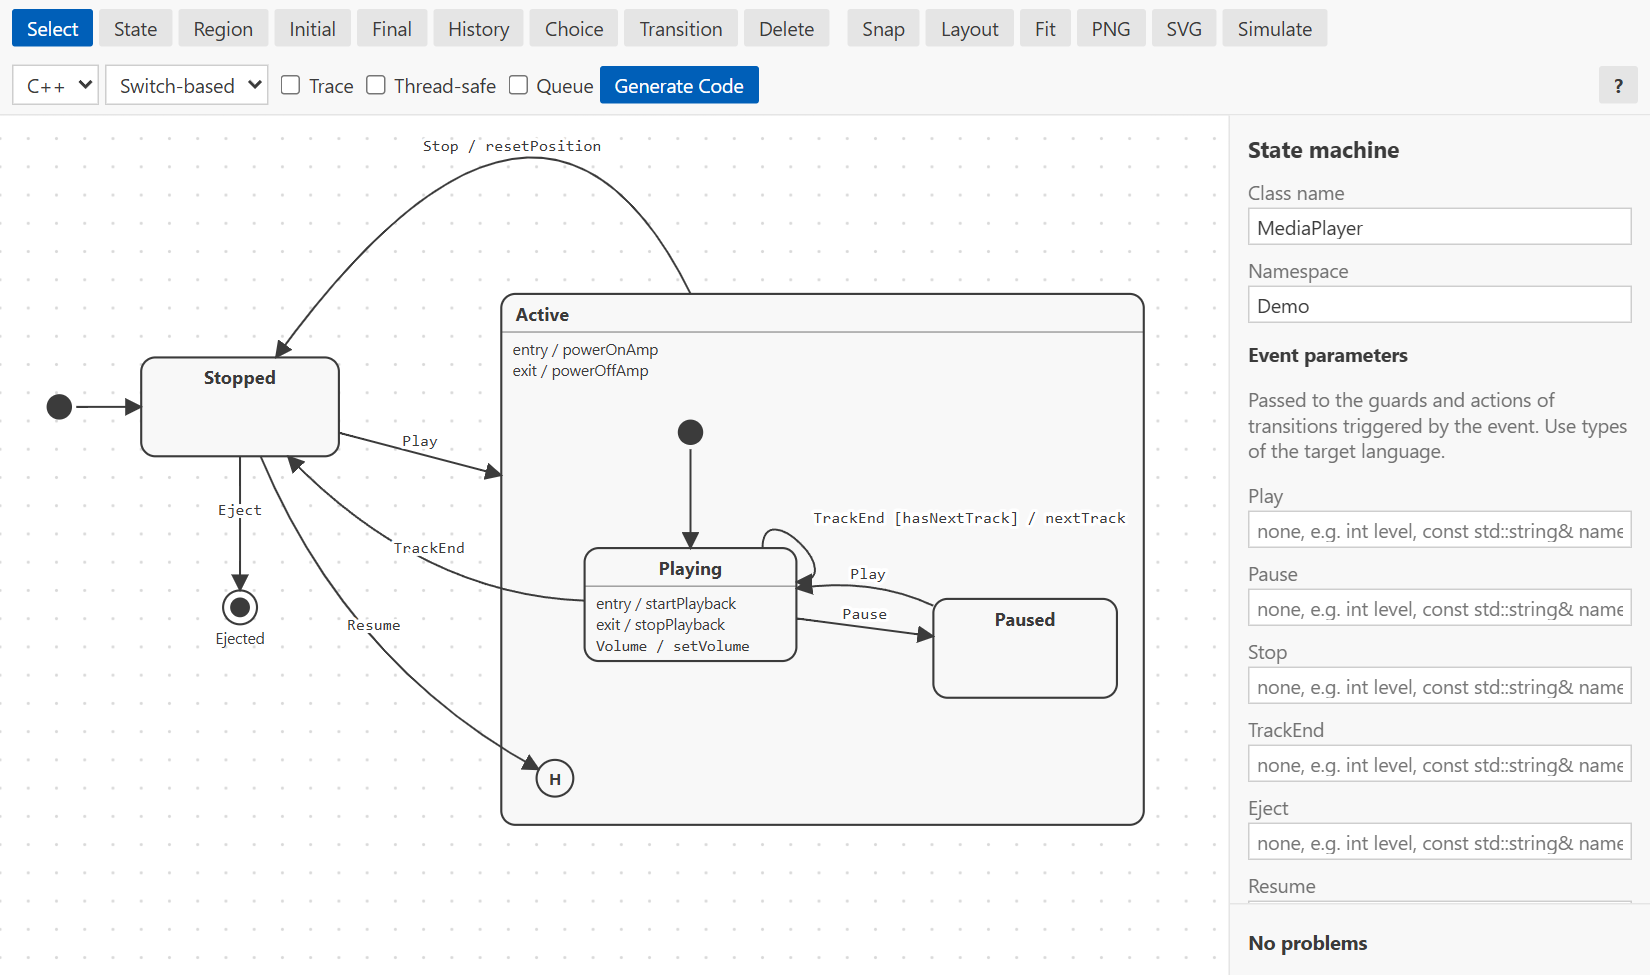
\includegraphics[width=\linewidth]{tour.png}};
  \begin{scope}[x={(img.south east)}, y={(img.north west)}]
    \node[callout] at (0.255, 0.94) {1};
    \node[callout] at (0.659, 0.94) {2};
    \node[callout] at (0.475, 0.913) {3};
    \node[callout] at (0.036, 0.79) {4};
    \node[callout] at (0.733, 0.85) {5};
    \node[callout] at (0.733, 0.034) {6};
    \node[callout] at (0.37, 0.68) {7};
    \node[callout] at (0.495, 0.338) {8};
    \node[callout] at (0.36, 0.20) {9};
  \end{scope}
\end{tikzpicture}
\caption{The diagram editor showing \code{examples/MediaPlayer.machina}.}
\label{fig:tour}
\end{figure}

\begin{enumerate}[label={\co{\arabic*}}, leftmargin=2.2em, itemsep=2pt]
  \item \textbf{Drawing tools.} \ui{Select} moves and resizes elements. \ui{State}, \ui{Region},
        \ui{Initial}, \ui{Final}, \ui{History} and \ui{Choice} add elements with a single click on the
        canvas;
        \ui{Transition} connects two elements by dragging. \ui{Delete} removes the selection.
  \item \textbf{View, export and simulation.} \ui{Snap} toggles the 10-pixel grid, \ui{Layout}
        arranges the diagram automatically, \ui{Fit} zooms to the whole diagram, \ui{PNG} and \ui{SVG} save an image and \ui{Simulate} starts the simulator. The \ui{?} button at the right end of the toolbar opens the help (Section~\ref{sec:help}).
  \item \textbf{Code generation options.} Target language (C++, C\# or C), implementation style, the optional
        \ui{Trace}, \ui{Thread-safe} and \ui{Queue} features, and the \ui{Generate Code} button.
  \item \textbf{Canvas.} Drag empty space to pan, use the mouse wheel to zoom.
  \item \textbf{Properties panel.} Shows the properties of the selected element --- or, with nothing
        selected, the class name, namespace and event parameters.
  \item \textbf{Problems list.} All validation problems; click one to select the element concerned.
        The same problems appear in VS Code's \ui{Problems} panel.
  \item \textbf{Composite state.} \code{Active} contains other states, its own initial pseudostate and
        a history pseudostate. Entry and exit actions are listed below the name.
  \item \textbf{Internal transition.} \code{Volume / setVolume} is handled inside \code{Playing}
        without leaving it.
  \item \textbf{History pseudostate.} The \code{Resume} transition re-enters \code{Active} in the
        substate that was active when it was left.
\end{enumerate}

\section{The toolbar}
\begin{figure}[H]
  \centering
  \fbox{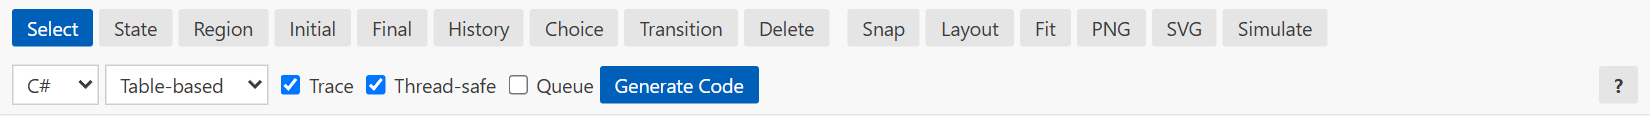
\includegraphics[width=0.985\linewidth]{toolbar.png}}
  \caption{The toolbar with C\#, table-based, \ui{Trace} and \ui{Thread-safe} selected. In a narrow
  window the toolbar wraps onto two rows.}
\end{figure}
The language, style and the three check boxes are stored in the diagram, so everyone who opens the file
generates the same code. Chapter~\ref{ch:editor} describes every button in detail.

\section{Diagram notation}
MachinaState uses standard UML notation (Figure~\ref{fig:notation}).

\begin{figure}[H]
\centering
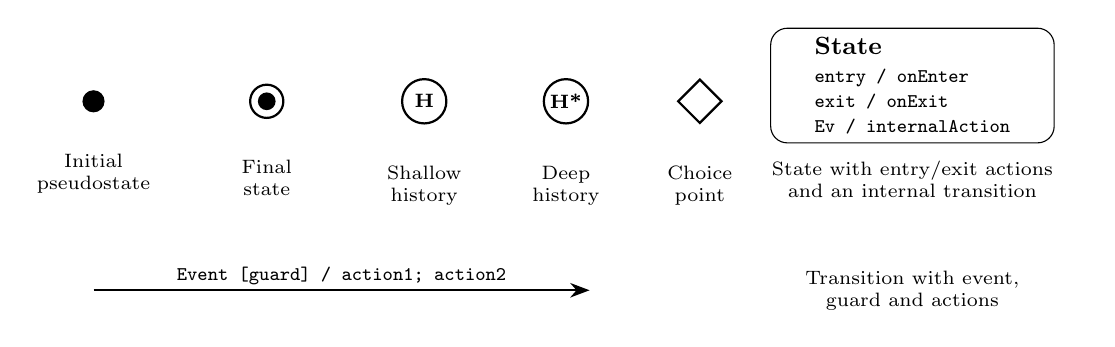
\begin{tikzpicture}[every node/.style={font=\small}]
  \node[init] (a) at (0,0) {}; \node[below=4mm of a, align=center, font=\scriptsize] {Initial\\pseudostate};
  \node[final] (b) at (2.2,0) {}; \node[below=4mm of b, align=center, font=\scriptsize] {Final\\state};
  \node[hist] (c) at (4.2,0) {H}; \node[below=4mm of c, align=center, font=\scriptsize] {Shallow\\history};
  \node[hist] (d) at (6.0,0) {H*}; \node[below=4mm of d, align=center, font=\scriptsize] {Deep\\history};
  \node[choicept] (ch) at (7.7,0) {}; \node[below=4mm of ch, align=center, font=\scriptsize] {Choice\\point};
  \node[st, align=left, minimum width=3.6cm] (e) at (10.4,0.2) {\textbf{State}\\[-1pt]\scriptsize\ttfamily entry / onEnter\\[-2pt]\scriptsize\ttfamily exit / onExit\\[-2pt]\scriptsize\ttfamily Ev / internalAction};
  \node[below=1mm of e, font=\scriptsize, align=center, text width=4.2cm] {State with entry/exit actions and an internal transition};
  \draw[tr] (0,-2.4) -- node[lbl, above]{Event [guard] / action1; action2} (6.3,-2.4);
  \node[font=\scriptsize, align=center, text width=4.2cm] at (10.4,-2.4) {Transition with event, guard and actions};
\end{tikzpicture}
\caption{Elements of the notation.}
\label{fig:notation}
\end{figure}

%=====================================================================
\part{Tutorials}

\chapter{Tutorial 1: A Traffic Light}
\label{ch:tut1}

In this tutorial you build the classic three-colour traffic light, simulate it and run it as a small
C++ program. It introduces the editing workflow; later tutorials build on it.

\begin{figure}[H]
\centering
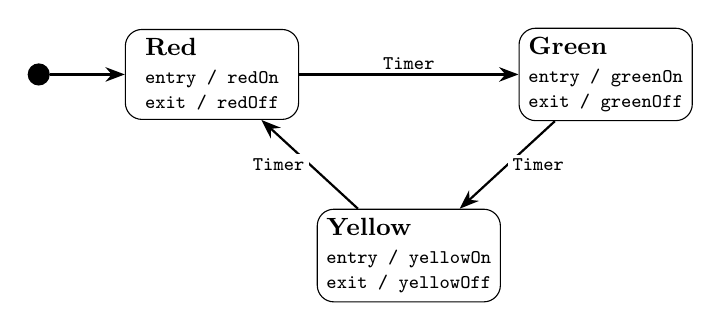
\begin{tikzpicture}
  \node[init] (i) at (0,0) {};
  \node[st, align=left] (r) at (2.2,0) {\textbf{Red}\\[-1pt]\scriptsize\ttfamily entry / redOn\\[-2pt]\scriptsize\ttfamily exit / redOff};
  \node[st, align=left] (g) at (7.2,0) {\textbf{Green}\\[-1pt]\scriptsize\ttfamily entry / greenOn\\[-2pt]\scriptsize\ttfamily exit / greenOff};
  \node[st, align=left] (y) at (4.7,-2.3) {\textbf{Yellow}\\[-1pt]\scriptsize\ttfamily entry / yellowOn\\[-2pt]\scriptsize\ttfamily exit / yellowOff};
  \draw[tr] (i) -- (r);
  \draw[tr] (r) -- node[lbl, above]{Timer} (g);
  \draw[tr] (g) -- node[lbl, right]{Timer} (y);
  \draw[tr] (y) -- node[lbl, left]{Timer} (r);
\end{tikzpicture}
\caption{Goal of Tutorial 1.}
\end{figure}

\section{Step 1 --- Create the diagram}
\begin{enumerate}
  \item Run \ui{MachinaState: New State Machine Diagram} and save it as \code{TrafficLight.machina}.
  \item The new diagram contains an initial pseudostate connected to a state named \code{Idle}.
        Double-click \code{Idle} and rename it to \code{Red}; press \key{Enter} to apply.
  \item With nothing selected (click on empty canvas), set \ui{Class name} to \code{TrafficLight} and
        \ui{Namespace} to \code{Demo}.
\end{enumerate}

\screenshot{t1-step1}{Step 1: the initial pseudostate points at \code{Red}. The \ui{State} tool is
active, ready to place the next state. The square at the bottom-right corner of the selected state
resizes it.}

\section{Step 2 --- Add the other states}
\begin{enumerate}
  \item Click \ui{State} in the toolbar and click on the canvas to the right of \code{Red}. A state
        named \code{State1} appears and is selected.
  \item Type \code{Green} in the \ui{Name} field and press \key{Enter}.
  \item Repeat for \code{Yellow}, placing it below and between the two.
\end{enumerate}
After adding an element, the editor switches back to the \ui{Select} tool so that you can immediately
move or edit it. Drag states by their body to arrange them.

\screenshot{t1-step2}{Step 2: three states, \code{Yellow} selected.}

\begin{tip}
State names become enumeration values in the generated code, so they must be valid identifiers and
unique within the whole diagram. The problems list tells you immediately if a name is not allowed.
\end{tip}

\section{Step 3 --- Connect the states}
\begin{enumerate}
  \item Click \ui{Transition}. Press the mouse button on \code{Red}, drag to \code{Green} and release.
  \item The new transition is selected and has the placeholder event \code{Event}. Change \ui{Event}
        to \code{Timer} and press \key{Enter}.
  \item Create \code{Green}\,$\rightarrow$\,\code{Yellow} and \code{Yellow}\,$\rightarrow$\,\code{Red}
        the same way, both with the event \code{Timer}.
\end{enumerate}

\screenshot{t1-step3}{Step 3: the \code{Red}\,$\rightarrow$\,\code{Green} transition is selected and
shows its properties.}

\begin{tip}
Drag a transition's label to curve it --- useful when two transitions connect the same states in
opposite directions. Drag the label back close to the straight line, or press \ui{Straighten}, to
make it straight again.
\end{tip}

\section{Step 4 --- Add entry and exit actions}
A light should switch on when its state is entered and off when it is left. Select \code{Red} and
enter \code{redOn} in \ui{Entry actions} and \code{redOff} in \ui{Exit actions}. Do the same for
\code{Green} (\code{greenOn}, \code{greenOff}) and \code{Yellow} (\code{yellowOn}, \code{yellowOff}).

\screenshot{t1-step4}{Step 4: \code{Red} with entry and exit actions.}

Actions are \emph{names} of methods. The generator declares each name as an abstract method in the
generated class, and you implement it later. To run several actions, separate them with semicolons:
\code{redOn; startTimer}.

\section{Step 5 --- Simulate}
Before writing any code, check that the machine behaves as intended.
\begin{enumerate}
  \item Click \ui{Simulate}. Editing is disabled, the machine is started, and \code{Red} is highlighted.
  \item The \ui{Events} list has a button for every event. Click \ui{Timer} twice.
  \item The \ui{Trace} shows each step: the event, the exit of the old state with its exit action, and
        the entry of the new state with its entry action.
\end{enumerate}

\screenshot{t1-sim}{Step 5: after two \code{Timer} events the light is \code{Yellow}. The transition
taken in the last step is highlighted.}

Click \ui{Reset} to start over or \ui{Stop} to return to editing.

\section{Step 6 --- Generate the code}
Select \ui{C++} and \ui{Switch-based} in the toolbar and click \ui{Generate Code}. MachinaState writes
\code{TrafficLight.hpp} next to the diagram and opens it beside the editor. The class looks like this
(abridged; Appendix~\ref{app:flat-switch} contains the full file):

\begin{lstlisting}[language=C++]
namespace Demo {
    class TrafficLight {
      public:
        enum class State { Red, Green, Yellow, None };
        enum class Event { Timer };

        void Start();                      // enter the initial state
        bool Dispatch(Event event);        // process one event
        State Current() const;             // innermost active state
        bool IsIn(State state) const;
        bool IsFinished() const;
        static const char* StateName(State state);
        static const char* EventName(Event event);

      protected:
        // Actions
        virtual void redOn() = 0;
        virtual void redOff() = 0;
        virtual void greenOn() = 0;
        // ...
    };
}
\end{lstlisting}

\section{Step 7 --- Use the generated class}
Create \code{main.cpp}, derive from \code{TrafficLight} and implement the six actions:

\lstinputlisting[language=C++]{examples/traffic_flat.cpp}

Compile and run it (the generated header was saved as \code{TrafficLightFlat\_switch.hpp} for this
manual):
\begin{lstlisting}[language=bash]
g++ -std=c++17 -Wall -Wextra -o traffic main.cpp && ./traffic
\end{lstlisting}

\lstinputlisting[style=output, caption={Output of the Tutorial 1 program.}]{generated/traffic_flat.txt}

\section{What you have learned}
\begin{itemize}[itemsep=1pt]
  \item Adding states and transitions, naming events and attaching entry and exit actions.
  \item Checking behaviour in the simulator before writing code.
  \item Generating a class and implementing its actions in a subclass.
\end{itemize}

%=====================================================================
\chapter{Tutorial 2: Hierarchy, History and Internal Transitions}
\label{ch:tut2}

Real traffic lights can be switched off and fall back to a flashing mode when a fault is detected.
After the repair they should continue with the colour they showed before. This tutorial extends the
traffic light with a \emph{composite state}, a \emph{history pseudostate} and an \emph{internal
transition}, and generates table-based C++ code with tracing.

\section{Step 1 --- Create the composite state}
\begin{enumerate}
  \item Open \code{TrafficLight.machina} from Tutorial~1 (or \code{examples/TrafficLight.machina},
        which contains the finished result).
  \item Click \ui{State} and add a new state \code{Operating} in an empty area. Resize it with the
        corner handle until it is large enough to hold the three colours.
  \item Drag \code{Red}, \code{Green} and \code{Yellow} into \code{Operating}. A state becomes a child of
        the state under its \emph{centre} when you drop it.
\end{enumerate}

\begin{tip}
You can also draw the large state \emph{around} existing states: when you resize a state so that a
sibling lies completely inside it, the sibling becomes its child.
\end{tip}

Every composite state needs its own initial pseudostate that defines the default substate:
\begin{enumerate}[resume]
  \item Select the old top-level initial pseudostate and move it into \code{Operating}, next to
        \code{Red}. It now belongs to \code{Operating}'s region.
  \item Add a new state \code{Off} outside \code{Operating}, then add a new initial pseudostate at the
        top level and connect it to \code{Off} with the \ui{Transition} tool.
\end{enumerate}

\section{Step 2 --- Power and fault handling}
\begin{enumerate}
  \item Connect \code{Off}\,$\rightarrow$\,\code{Operating} with the event \code{PowerOn}, and
        \code{Operating}\,$\rightarrow$\,\code{Off} with \code{PowerOff}.
  \item Add a top-level state \code{Flashing} with entry action \code{flashOn} and exit action
        \code{flashOff}.
  \item Connect \code{Operating} to \code{Flashing} with event \code{Fault} and action
        \code{logFault}, and \code{Flashing} to \code{Off} with \code{PowerOff}.
\end{enumerate}

Because \code{PowerOff} and \code{Fault} start at the \emph{composite} state \code{Operating}, they are
available no matter which colour is active: an event that the active substate does not handle
\emph{bubbles up} to its parent (Section~\ref{sec:dispatch}).

\section{Step 3 --- Resume with history}
\begin{enumerate}
  \item Click \ui{History} and click inside \code{Operating} to add a history pseudostate (\code{H}).
  \item Connect \code{Flashing} to \code{H} with the event \code{Repair}.
\end{enumerate}
A transition to \code{H} re-enters \code{Operating} in the colour that was active when
\code{Operating} was last left. Without history it would always restart at \code{Red}.

\screenshot{t2-history}{The history pseudostate is selected. \ui{Deep history (H*)} would resume the
innermost state instead of the direct substate; both behave the same here because the colours have no
substates of their own.}

\section{Step 4 --- An internal transition}
Pedestrians can request a shorter green phase. The request must not restart the green phase --- which
an ordinary self transition would do, running \code{greenOff} and \code{greenOn}.
\begin{enumerate}
  \item With the \ui{Transition} tool, drag from \code{Green} back onto \code{Green} to create a self
        transition.
  \item Set \ui{Event} to \code{PedestrianRequest} and \ui{Action} to \code{shortenGreen}.
  \item Tick \ui{Internal (no exit / entry)}. The loop disappears and the transition is listed inside
        \code{Green} instead.
\end{enumerate}

\screenshot{t2-internal}{The internal transition is selected by clicking its line inside \code{Green}.}

The finished diagram is shown in Figure~\ref{fig:t2-final}.

\screenshot{t2-final}{The hierarchical traffic light (\code{examples/TrafficLight.machina}).}

\section{Step 5 --- Simulate the fault scenario}
Start the simulator and fire \code{PowerOn}, \code{Timer}, \code{Fault} and \code{Repair}. The trace
shows that \code{Fault} exits \code{Green} \emph{and} \code{Operating} before entering \code{Flashing},
and that \code{Repair} resumes \code{Green} from history: it is traced as
\code{transition Flashing -> Operating (history)}, followed directly by \code{enter Green}.

\screenshot{t2-sim}{After \code{Repair} the light is green again, resumed from history.}

\section{Step 6 --- Generate table-based code with tracing}
Select \ui{C++}, \ui{Table-based}, tick \ui{Trace} and click \ui{Generate Code}. The table-based class
keeps the hierarchy, entry/exit handlers and transitions in constant arrays. The core of
\code{Dispatch} is a short loop over the transition table, and \code{TryRow} fires a matching row:

\lstinputlisting[language=C++, caption={\code{HandleEvent} in the table-based flat traffic
light.}]{generated/snippets/table-handle.hpp}

\lstinputlisting[language=C++, caption={\code{TryRow}: guard check, exit, action,
entry.}]{generated/snippets/table-tryrow.hpp}

With history, \code{ExitState} records in an array the state that was last exited from each region,
so the array always describes the configuration that every composite state had when it was last left.
A transition to the history pseudostate enters \code{Operating} through \code{EnterHistory}, which
re-enters the recorded substate instead of following the initial transition:

\lstinputlisting[language=C++, caption={History restoration in the generated hierarchical traffic
light.}]{generated/snippets/history.hpp}

\section{Step 7 --- Run it}
The program below implements the hooks and the \code{Trace} method and plays the same scenario as the
simulator, followed by \code{PowerOff}.

\lstinputlisting[language=C++]{examples/traffic_nested.cpp}

\lstinputlisting[style=output, caption={Output of the Tutorial 2 program.}]{generated/traffic_nested.txt}

Compare the output with the simulator trace in Figure~\ref{fig:t2-sim}: they describe the same
sequence of exits, actions and entries. Note in particular:
\begin{itemize}[itemsep=1pt]
  \item \code{PowerOn} enters \code{Operating} and then follows its initial transition to \code{Red}.
  \item \code{PedestrianRequest} only calls \code{shortenGreen()} --- no exit, no entry.
  \item \code{Fault} exits the innermost state first (\code{Green}, then \code{Operating}), runs the
        transition action \code{logFault()}, and only then enters \code{Flashing}.
  \item \code{Repair} enters \code{Operating} and resumes \code{Green} instead of \code{Red}.
\end{itemize}

%=====================================================================
\chapter{Tutorial 3: A Thread-Safe Door Lock in C\#}
\label{ch:tut3}

This tutorial builds an electronic door lock that is opened with a numeric code. It shows
\emph{event parameters}, \emph{guards}, transition priority, and the optional \emph{tracing} and
\emph{thread safety} features, using C\# and the table-based style.

\begin{figure}[H]
\centering
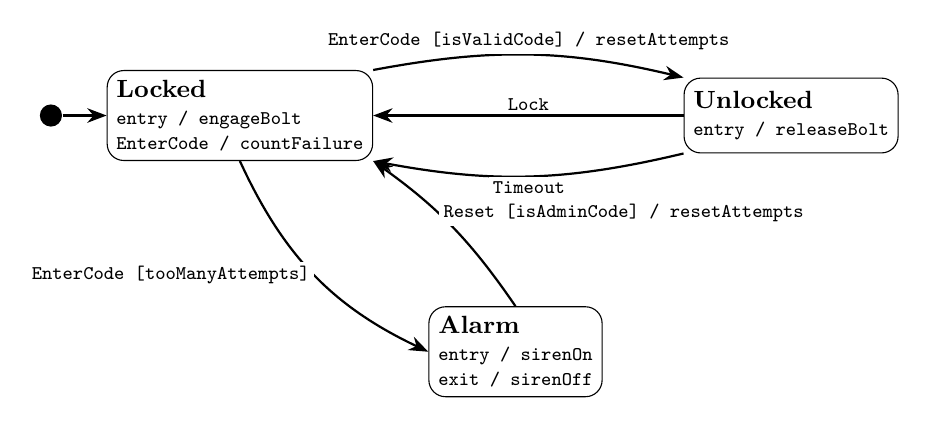
\begin{tikzpicture}
  \node[init] (i) at (-0.4,0) {};
  \node[st, align=left] (l) at (2,0) {\textbf{Locked}\\[-1pt]\scriptsize\ttfamily entry / engageBolt\\[-2pt]\scriptsize\ttfamily EnterCode / countFailure};
  \node[st, align=left] (u) at (9,0) {\textbf{Unlocked}\\[-1pt]\scriptsize\ttfamily entry / releaseBolt};
  \node[st, align=left] (a) at (5.5,-3) {\textbf{Alarm}\\[-1pt]\scriptsize\ttfamily entry / sirenOn\\[-2pt]\scriptsize\ttfamily exit / sirenOff};
  \draw[tr] (i) -- (l);
  \draw[tr] (l.north east) to[bend left=12] node[lbl, above]{EnterCode [isValidCode] / resetAttempts} (u.north west);
  \draw[tr] (u.west) -- node[lbl, above]{Lock} (l.east);
  \draw[tr] (u.south west) to[bend left=12] node[lbl, below]{Timeout} (l.south east);
  \draw[tr] (l.south) to[bend right=20] node[lbl, left]{EnterCode [tooManyAttempts]} (a.west);
  \draw[tr] (a.north) to[bend right=10] node[lbl, right, pos=0.6]{Reset [isAdminCode] / resetAttempts} (l.south east);
\end{tikzpicture}
\caption{Goal of Tutorial 3 (\code{examples/DoorLock.machina}).}
\end{figure}

\section{Step 1 --- States and transitions}
Create a new diagram \code{DoorLock.machina} with class name \code{DoorLock} and namespace
\code{Security}, and draw the states and transitions shown above:
\begin{itemize}[itemsep=1pt]
  \item \code{Locked} (entry \code{engageBolt}), \code{Unlocked} (entry \code{releaseBolt}) and
        \code{Alarm} (entry \code{sirenOn}, exit \code{sirenOff}).
  \item Two transitions from \code{Locked} with the event \code{EnterCode}: to \code{Unlocked} with guard
        \code{isValidCode} and action \code{resetAttempts}, and to \code{Alarm} with guard
        \code{tooManyAttempts}.
  \item An internal transition in \code{Locked}: \code{EnterCode / countFailure}.
  \item \code{Unlocked}\,$\rightarrow$\,\code{Locked} with \code{Lock} and with \code{Timeout};
        \code{Alarm}\,$\rightarrow$\,\code{Locked} with \code{Reset [isAdminCode] / resetAttempts}.
\end{itemize}

\screenshot{t3-guard}{The guarded transition \code{EnterCode [isValidCode] / resetAttempts}.}

\section{Step 2 --- Understand the priority of guarded transitions}
\code{Locked} now has three transitions for \code{EnterCode}. When the event arrives, MachinaState
tries them in a fixed order:
\begin{enumerate}[itemsep=1pt]
  \item guarded transitions first, in the order they appear in the diagram --- \code{[isValidCode]},
        then \code{[tooManyAttempts]};
  \item then the unguarded one --- the internal \code{countFailure}.
\end{enumerate}
The first transition whose guard is true fires. A wrong code therefore falls through both guards
and is counted by \code{countFailure}; after too many failures \code{tooManyAttempts} becomes true and
the alarm goes off. A state may have at most one unguarded transition per event, because a second
one could never fire.

\section{Step 3 --- Event parameters}
The guards need to see the code that was entered. Click on empty canvas to show the machine
properties. Under \ui{Event parameters}, enter \code{int code} for \code{EnterCode} and for
\code{Reset}.

\screenshot{t3-params}{Event parameters are declared once per event in the machine properties.}

All guards and actions of transitions triggered by \code{EnterCode} now receive the parameter:
\code{isValidCode(int code)}, \code{tooManyAttempts(int code)}, \code{resetAttempts(int code)} and
\code{countFailure(int code)}. Write parameter types in the syntax of the language you generate ---
\code{int code} is valid in both C++ and C\#, while e.g. \code{const std::string\& name} is C++ only.

\section{Step 4 --- Simulate}
Because the simulator cannot run your code, \emph{you} decide what each guard returns: the
\ui{Guard results} list has a check box per guard. Untick \ui{isValidCode} and
\ui{tooManyAttempts}, type a code into the argument field of \code{EnterCode} and fire it twice ---
both guards are false, so the internal transition counts the failures. Then tick \ui{isValidCode}
and fire \code{EnterCode} with \code{1234}. The trace shows every guard call with its argument and
result:

\screenshot{t3-sim}{Two failed attempts are counted, then the valid code unlocks the door.}

\section{Step 5 --- Generate C\# with tracing and thread safety}
Select \ui{C\#}, \ui{Table-based}, tick \ui{Trace} and \ui{Thread-safe}, and click \ui{Generate Code}.
The interesting parts of the generated \code{DoorLock.cs}:

\lstinputlisting[language={[Sharp]C}, caption={The transition table is built in the constructor.
Arguments are passed to hooks from fields set by the typed dispatch method.}]{generated/snippets/doorlock-table.cs}

\lstinputlisting[language={[Sharp]C}, caption={Each event with parameters gets a typed dispatch
method. \code{Lock}/\code{Unlock} surround every public member.}]{generated/snippets/doorlock-dispatch.cs}

The hooks you must implement:
\lstinputlisting[language={[Sharp]C}, caption={The hooks to implement.}]{generated/snippets/doorlock-hooks.cs}

\section{Step 6 --- Implement and run}
\lstinputlisting[language={[Sharp]C}, caption={\code{Program.cs} of the door lock demo.}]{examples/DoorLockDemo/Program.cs}

\lstinputlisting[style=output, caption={Output of the Tutorial 3 program. The order of the last four
events depends on thread scheduling.}]{generated/doorlock.txt}

Notice:
\begin{itemize}[itemsep=1pt]
  \item \code{Dispatch(Event.EnterCode)} returns \code{false} --- events with parameters must be sent
        with their typed method \code{DispatchEnterCode(int)}.
  \item While the alarm sounds, \code{Lock} is \emph{ignored} because no active state handles it.
  \item \code{Parallel.For} calls \code{Dispatch} from several threads; \code{Lock()}/\code{Unlock()}
        make each call atomic.
\end{itemize}

%=====================================================================
\chapter{Tutorial 4: A Vending Machine with Choices, Timeouts and a Queue}
\label{ch:tut4}

The last tutorial uses the newest modelling elements. The vending machine collects coins until the
credit covers the price, dispenses the selected item, returns change, and gives up after 30 seconds
without a coin. You will meet:
\begin{itemize}[itemsep=1pt]
  \item a \textbf{completion transition} that leaves \code{Boot} as soon as it has been entered;
  \item a \textbf{choice point} that branches on the credit, shared by two incoming transitions;
  \item \textbf{timeouts} with \code{after(30s)} and \code{after(2s)};
  \item the \textbf{completion of a composite state} when its region reaches a final state;
  \item the \textbf{event queue}, used by an action to raise a follow-up event.
\end{itemize}
The finished diagram is \code{examples/VendingMachine.machina} (Figure~\ref{fig:t4-overview}).

\screenshot{t4-overview}{The finished vending machine.}

\section{Step 1 --- Boot with a completion transition}
Add an initial pseudostate, a state \code{Boot} with entry action \code{selfTest} and a state
\code{Idle} with entry action \code{showWelcome}. Connect \code{Boot} to \code{Idle} and
\emph{clear the event field}. A transition without an event is a \emph{completion transition}: it
fires on its own as soon as \code{Boot} has been entered (and its entry action has run). There is no
need for an artificial ``BootDone'' event.

\section{Step 2 --- Collect coins through a choice point}
Pick the \ui{Choice} tool and place a diamond to the right of \code{Idle}. Add the states
\code{Collecting} (entry \code{showCredit}) and \code{Ready} (entry \code{showSelect}) and connect:
\begin{enumerate}[itemsep=1pt]
  \item \code{Idle}\,$\rightarrow$\,choice with event \code{Coin} and action \code{addCredit};
  \item \code{Collecting}\,$\rightarrow$\,choice with the same event and action;
  \item choice\,$\rightarrow$\,\code{Ready} with guard \code{hasEnoughCredit};
  \item choice\,$\rightarrow$\,\code{Collecting} with guard \code{else}.
\end{enumerate}
Branches leaving a choice point have no event; the \ui{Event} field is disabled for them. The
\code{[else]} branch is taken when no other guard is true (Figure~\ref{fig:t4-choice}).

\screenshot{t4-choice}{The \code{[else]} branch of the choice point is selected.}

With nothing selected, enter the parameter list \code{int cents} for \code{Coin} and \code{int item}
for \code{Select}. Because the choice branches belong to transitions triggered by \code{Coin}, the
guard is generated as \code{hasEnoughCredit(int cents)} as well.

\begin{note}
MachinaState evaluates the guards of a choice point \emph{before} the transition starts, i.e. before
any state is exited and before \code{addCredit} runs. The guard therefore has to add the incoming coin
itself: \code{credit + cents >= price}. Section~\ref{sec:choice} explains why.
\end{note}

\section{Step 3 --- Give up after 30 seconds}
Connect \code{Collecting}\,$\rightarrow$\,\code{Idle} with the event \code{after(30s)} and the action
\code{refund}. A timeout is written as \code{after(}\textit{n}\,\code{ms}\,|\,\code{s}\,|\,\code{min)}.
The generated code starts a timer whenever \code{Collecting} is entered and cancels it whenever
\code{Collecting} is left --- so every coin, which leaves and re-enters \code{Collecting} through the
choice point, restarts the 30 seconds (Figure~\ref{fig:t4-timeout}).

\screenshot{t4-timeout}{A timeout transition.}

\section{Step 4 --- Dispense, then return change}
Add a composite state \code{Dispensing} (entry \code{openFlap}, exit \code{closeFlap}) containing an
initial pseudostate, a state \code{Dropping} and a final state \code{Done}, with
\code{Dropping}\,$\rightarrow$\,\code{Done} on \code{after(2s)}. Connect:
\begin{itemize}[itemsep=1pt]
  \item \code{Ready}\,$\rightarrow$\,\code{Dispensing} on \code{Select [inStock] / vend};
  \item \code{Ready}\,$\rightarrow$\,\code{Idle} on \code{Cancel / refund};
  \item an internal transition \code{Coin / addCredit} on \code{Ready} (draw a self transition and
        tick \ui{Internal});
  \item a completion transition from \code{Dispensing} to a second choice point with the branches
        \code{[hasChange] / giveChange} and \code{[else]}, both to \code{Idle}.
\end{itemize}
The completion transition of \code{Dispensing} fires when its region reaches \code{Done}.

\section{Step 5 --- Simulate}
Press \ui{Simulate}. The simulator starts the machine like \code{Start()} does: \code{Boot} is entered,
\code{selfTest} runs, and the completion transition takes the machine straight on to \code{Idle}.

The simulator cannot run your guard methods, so it lists every guard under \ui{Guard results} with a
check box: ticked means the guard returns \code{true}. Untick \ui{hasEnoughCredit}, type \code{100}
into the argument field next to \ui{Coin} and click \ui{Coin}. The transition reaches the choice
point, \code{[hasEnoughCredit]} is false, so the \code{[else]} branch leads back to \code{Collecting}
(Figure~\ref{fig:t4-sim-choice}). Entering \code{Collecting} started its 30-second timer, which now
appears under \ui{Running timers}; clicking it lets the timer elapse.

\screenshot{t4-sim-choice}{The \code{[else]} branch was taken. The timer of \code{Collecting} is
running; the trace shows the guard result next to the guard call.}

Now tick \ui{hasEnoughCredit}, fire \code{Coin} with \code{50} and \code{Select} with \code{1}, and
click \ui{after 2 s}. Entering the final state \code{Done} completes \code{Dispensing}; its completion
transition runs through the second choice point and, since \code{hasChange} is ticked, calls
\code{giveChange} on the way to \code{Idle} --- all within the same step, exactly as in the generated
code (Figure~\ref{fig:t4-sim-completion}).

\screenshot{t4-sim-completion}{\code{Dispensing} has completed and the machine is back in
\code{Idle}. With \ui{Highlight untaken}, the transitions not yet covered are drawn in red.}

The coverage counter shows how many transitions have been taken since the simulation started. Tick
\ui{Highlight untaken} to see the rest in red: here the timeout, \code{Cancel}, the internal
\code{Coin} of \code{Ready} and the \code{[else]} branch of the change point are still untested.

\section{Step 6 --- Generate with trace and queue}
Select \ui{C++} and \ui{Switch-based}, tick \ui{Trace} and \ui{Queue}, and click \ui{Generate Code}.
Besides the guard and action hooks, the class now requires two timer hooks and offers \code{Post}:
\begin{lstlisting}[language=C++]
virtual void StartTimer(Event timeout, unsigned milliseconds, unsigned generation) = 0;
virtual void CancelTimer(Event timeout)                                            = 0;
bool DispatchTimeout(Event timeout, unsigned generation);  // public: report an elapsed timer
bool Post(Event event);                    // protected: queue an event from a hook
bool PostCoin(int cents);                  // typed variant for events with parameters
\end{lstlisting}
Timeouts are events with generated names such as \code{Collecting\_After30000ms}. When a timer
elapses, your code calls \code{DispatchTimeout} with the event and the \code{generation} number it was
given by \code{StartTimer}. The machine ignores the call if the timer has been cancelled or restarted
in the meantime, or if that timeout has already been dispatched, so a late timer can never fire a newer
one early (Section~\ref{sec:timers}).

\section{Step 7 --- Implement and run}
The program uses a fake timer that main() lets ``elapse''. It also shows the queue: when the credit
exceeds a limit, \code{addCredit} posts \code{Cancel}, which is processed right after the current
\code{Coin} has been handled.

\lstinputlisting[language=C++, caption={\code{vending.cpp}.}]{examples/vending.cpp}

\lstinputlisting[style=output, caption={Output of the Tutorial 4 program.}]{generated/vending.txt}

Observe:
\begin{itemize}[itemsep=1pt]
  \item the completion transition \code{Boot -> Idle} fires inside \code{Start()};
  \item the choice transitions are traced as \code{(choice)} and exit the source before running
        \code{addCredit};
  \item \code{StartTimer}/\code{CancelTimer} bracket the time spent in \code{Collecting} and
        \code{Dropping}; the second visit to \code{Collecting} starts its timer with generation 2;
  \item reaching \code{Done} immediately triggers the completion of \code{Dispensing};
  \item the posted \code{Cancel} is dispatched after the internal \code{Coin} transition has completed
        --- never in the middle of it.
\end{itemize}

%=====================================================================
\chapter{Tutorial 5: A Washing Machine with Orthogonal Regions}
\label{ch:tut5}

A washing machine does several things at once: the drum runs through its programme while the heater
keeps the water at temperature. Modelling both in one chain of states would need a state for every
combination (\code{Washing+Heating}, \code{Washing+Holding}, \code{Rinsing+Heating}, \dots). UML
\emph{orthogonal regions} keep them apart: a state is divided into regions, and while the state is
active, \emph{each} of its regions has its own active substate. This tutorial builds
\code{examples/Washer.machina} (Figure~\ref{fig:t5-overview}) and then uses \emph{scenarios} to turn
simulator sessions into repeatable tests. You will meet:
\begin{itemize}[itemsep=1pt]
  \item the \textbf{Region} tool and orthogonal states;
  \item events that are handled by \textbf{several regions at once};
  \item the \textbf{completion of an orthogonal state} once every region has finished;
  \item transitions that \textbf{leave all regions} at once, from the state or from inside one region;
  \item \textbf{scenarios}: recording, saving, replaying and stepping;
  \item \textbf{transition coverage}.
\end{itemize}

\screenshot{t5-overview}{The finished washing machine. \code{Running} has two regions, \code{Program}
and \code{Heater}.}

\section{Step 1 --- The outer states}
Create a new diagram with the class name \code{Washer} and the namespace \code{Appliances}. Add an
initial pseudostate, a state \code{Idle}, a large state \code{Running} (entry \code{lockDoor}, exit
\code{unlockDoor}) and a state \code{Error} (entry \code{alarm}). Connect \code{Idle} to
\code{Running} with \code{Start / fillWater}.

\section{Step 2 --- Divide Running into two regions}
Pick the \ui{Region} tool and click inside \code{Running}: a dashed rectangle appears. Click again
below it for the second region. Select each region and name it --- \code{Program} and \code{Heater}
(Figure~\ref{fig:t5-region}). Region names appear in the diagram and the generated comments; they do
not have to be identifiers. Resize the regions so that they fill \code{Running}; a region can only be
placed inside a state, and once a state has regions, all of its substates must be placed inside one
of them.

\screenshot{t5-region}{The \code{Heater} region is selected. Its properties name the orthogonal state
it belongs to.}

\section{Step 3 --- Fill the regions}
Each region is a small state machine of its own and needs its own initial pseudostate:
\begin{itemize}[itemsep=1pt]
  \item \textbf{Program}: \code{Washing} (entry \code{motorSlow}) $\rightarrow$ \code{Rinsing} on
        \code{after(30s) / drain}, $\rightarrow$ \code{Spinning} (entry \code{motorFast}, exit
        \code{motorStop}) on \code{after(20s)}, and $\rightarrow$ the final state \code{ProgramDone}
        on \code{Spun}.
  \item \textbf{Heater}: an initial transition with the action \code{setTemperature} to
        \code{Heating} (entry \code{heaterOn}, exit \code{heaterOff}); \code{Heating}
        $\rightarrow$ \code{Holding} on \code{TempReached} and back on \code{TempDropped}; an internal
        transition \code{SetTemp / adjust} on \code{Holding} with the parameter \code{int celsius};
        and \code{Holding} $\rightarrow$ the final state \code{HeaterDone} on \code{Spun}.
\end{itemize}
Note that \code{Spun} appears in both regions. An event is offered to every active region, so one
\code{Spun} finishes the programme and switches off the heater in the same step.

\section{Step 4 --- Leaving the orthogonal state}
Add four more transitions:
\begin{itemize}[itemsep=1pt]
  \item a \textbf{completion transition} \code{Running}\,$\rightarrow$\,\code{Idle} with the action
        \code{beep}. An orthogonal state completes when \emph{every} region has reached a final state,
        so it fires only after both \code{ProgramDone} and \code{HeaterDone};
  \item \code{Running}\,$\rightarrow$\,\code{Idle} on \code{Cancel / drain}: from the orthogonal state
        itself, it leaves both regions whatever their state;
  \item \code{Heating}\,$\rightarrow$\,\code{Error} on \code{Overheat}: a transition from inside one
        region to a state outside \code{Running} also exits the other region;
  \item \code{Error}\,$\rightarrow$\,\code{Idle} on \code{Reset [isCool]}, and
        \code{Idle}\,$\rightarrow$\,\code{Rinsing} on \code{QuickRinse}. Entering \code{Running}
        through a substate of one region starts the other regions at their initial states (the
        regions are still entered in their order, \code{Program} first).
\end{itemize}
Transitions \emph{between} the regions of one state are not allowed: the regions are independent by
definition. History pseudostates are not available in states with several regions; a deep history
pseudostate in an enclosing state does restore all of their regions (Section~\ref{sec:history}).

\section{Step 5 --- Simulate}
Press \ui{Simulate}, then fire \code{Start}, \code{TempReached} and the running timer
\ui{after 30 s} (Figure~\ref{fig:t5-sim}). \ui{Active} now lists one path per region,
\code{Running > Rinsing | Running > Holding}, and both active leaves are highlighted. The trace shows
the order of entry: \code{Running} and its entry action first, then the regions in order --- the
\code{Program} region enters \code{Washing}, then the \code{Heater} region runs its initial action
\code{setTemperature} and enters \code{Heating}. On the way out the order is reversed: the regions
are exited last-to-first, each innermost-first, before \code{Running} itself.

\screenshot{t5-sim}{Both regions are active: \code{Rinsing} in \code{Program} and \code{Holding} in
\code{Heater}. The 20-second timer of \code{Rinsing} is running.}

Now fire \code{Spun}. Only the \code{Heater} region handles it --- \code{Program} is still in
\code{Rinsing}, which has no \code{Spun} transition --- so the heater finishes in \code{HeaterDone}
while the drum carries on. Let \ui{after 20 s} elapse and fire \code{Spun} again: \code{Program}
reaches \code{ProgramDone}, every region has now finished, and the completion transition returns to
\code{Idle} with \code{beep}.

\section{Step 6 --- Record and replay scenarios}
Clicking through the same sequence after every change to the diagram is tedious. Instead, record it:
\begin{enumerate}[itemsep=1pt]
  \item Click \ui{Record}. The simulation restarts and the button changes to \ui{Save (0)}.
  \item Fire the events of the test case --- with the event arguments and guard results it needs.
        The counter on the button counts the recorded steps.
  \item Click \ui{Save}. The steps are stored in the diagram as a \emph{scenario} named
        \code{Scenario 1}, together with the arguments and the guards that were unticked. Rename it in
        the \ui{Scenarios} list; \ui{Discard} stops recording without saving.
\end{enumerate}
\ui{Run} restarts the simulation and replays all steps of a scenario; \ui{Step} restarts it and
replays one step per click, so you can watch each transition. The example contains two scenarios,
\code{Full program} and \code{Overheat}. Run \code{Full program} and tick \ui{Highlight untaken}
(Figure~\ref{fig:t5-scenario}): 9 of the 13 transitions were taken. The red ones --- \code{Cancel},
\code{QuickRinse}, \code{Overheat} and \code{Reset} --- are exactly what the \code{Overheat} scenario
covers apart from \code{Cancel}; run it as well and the coverage rises to 12/13. As an exercise,
record a third scenario that cancels a running programme to reach 13/13. Coverage accumulates until you press
\ui{Clear} or stop the simulator.

\screenshot{t5-scenario}{After replaying \code{Full program}: the trace ends with both regions
finishing and the completion transition to \code{Idle}. Untaken transitions are red.}

\begin{tip}
Scenarios are saved in the \code{.machina} file, so they travel with the diagram through version
control. After changing the diagram, replay the scenarios: a trace that changed unexpectedly, or a
scenario that no longer reaches the end, points straight at the regression. The trace of a replayed
scenario is the same trace the generated code produces with \ui{Trace} enabled.
\end{tip}

\section{Step 7 --- Generate}
Select \ui{C\#}, tick \ui{Trace} and generate. Regions change little in the interface:
\begin{itemize}[itemsep=1pt]
  \item \code{IsIn(State.Heating)} tells whether a state is active in any region;
  \item \code{Current} follows the \emph{first} region of an orthogonal state (\code{Program} here);
        use \code{IsIn} for the others;
  \item internally the class keeps one active state per region, and every hook runs in the order shown
        by the simulator trace.
\end{itemize}
The C++ and C generators produce the same structure, with fixed-size arrays and no allocation.

%=====================================================================
\part{Reference}

\chapter{Editor Reference}
\label{ch:editor}

\section{Toolbar}
\begin{longtable}{@{}p{3.1cm}p{11.3cm}@{}}
\toprule
\textbf{Control} & \textbf{Purpose} \\
\midrule
\endhead
\ui{Select}        & Select, move and resize elements; drag transition labels to bend transitions. \\
\ui{State}         & Click on the canvas to add a state. Clicking inside an existing state nests the new state. \\
\ui{Region}        & Click inside a state to add an orthogonal region to it (Section~\ref{sec:regions}). \\
\ui{Initial}       & Add an initial pseudostate (the black dot that marks a region's default state). \\
\ui{Final}         & Add a final state. \\
\ui{History}       & Add a history pseudostate inside a composite state (Section~\ref{sec:history}). \\
\ui{Choice}        & Add a choice point (Section~\ref{sec:choice}). \\
\ui{Transition}    & Press on the source element, drag to the target and release. Dragging from a state onto itself creates a self transition. \\
\ui{Delete}        & Delete the selection. Deleting a state also deletes its contents and all connected transitions. \\
\ui{Snap}          & Toggle snapping of positions and sizes to a 10-pixel grid. The setting is remembered per editor. The dot grid shows the snap positions and pans and zooms with the diagram; zoomed out, only every 2nd, 5th or 10th position is drawn. \\
\ui{Layout}        & Arrange all states and transitions automatically (Section~\ref{sec:layout}). This is a normal edit and can be undone. \\
\ui{Fit}           & Zoom and pan so that the whole diagram is visible. \\
\ui{PNG}, \ui{SVG}  & Save the whole diagram as a PNG or SVG image (Section~\ref{sec:export}). \\
\ui{Simulate}      & Start or stop the simulator (Chapter~\ref{ch:sim}). \\
Language           & \ui{C++}, \ui{C\#} or \ui{C}. \\
Style              & \ui{Switch-based} or \ui{Table-based} (Section~\ref{sec:styles}). \\
\ui{Trace}         & Generate a \code{Trace} method (Section~\ref{sec:trace}). \\
\ui{Thread-safe}   & Generate \code{Lock}/\code{Unlock} hooks around the public interface (Section~\ref{sec:threads}). \\
\ui{Queue}         & Generate \code{Post} so hooks can queue events (Section~\ref{sec:queue}). \\
\ui{Generate Code} & Generate code with the current options (Chapter~\ref{ch:codegen}). \\
\ui{?}             & At the right end of the toolbar: show the help dialog (Section~\ref{sec:help}). \\
\bottomrule
\end{longtable}

\section{Mouse and keyboard}
\begin{longtable}{@{}p{5cm}p{9.4cm}@{}}
\toprule
\textbf{Gesture} & \textbf{Effect} \\
\midrule
\endhead
Click an element                   & Selects it and shows its properties. \\
\key{Shift}/\key{Ctrl}+click a state & Adds it to (or removes it from) the selection. \\
\key{Shift}+drag on empty canvas    & Selects all elements inside the rectangle. \\
Drag a state                       & Moves the state --- or all selected states --- together with everything nested inside. \\
Drop a state inside another        & Makes it a substate of the state under its centre. \\
Drag a state out of its parent     & Moves it to the enclosing level. \\
Drag the corner handle             & Resizes the selected state. Siblings that end up fully inside it become its children; children whose centre ends up outside it leave it and are nested where they now lie. \\
Drag a transition label            & Bends the transition; near the straight line it snaps back to straight. \\
Double-click a state               & Selects it and focuses the \ui{Name} field. \\
Drag empty canvas / middle button  & Pans the view. \\
Mouse wheel                        & Zooms around the mouse pointer. \\
\key{Delete} / \key{Backspace}     & Deletes the selection. \\
\key{Ctrl}+\key{C} / \key{Ctrl}+\key{X} / \key{Ctrl}+\key{V} & Copies, cuts and pastes the selected states with their contents and the transitions between them --- also into another diagram. Names that already exist get a number appended. \\
\key{Ctrl}+\key{D}                 & Duplicates the selection. \\
\key{Ctrl}+\key{A}                 & Selects all top-level elements. \\
Arrow keys                         & Nudge the selection by 1 pixel (10 with \ui{Snap}); with \key{Shift} by 50 pixels. A burst of key presses is one undo step, and nudged states are nested where they end up, as after a drag. \\
\key{Esc}                          & Cancels the current tool and clears the selection. \\
\key{Ctrl}+\key{Z} / \key{Ctrl}+\key{Y} & Undo / redo (handled by VS Code). \\
\key{Ctrl}+\key{S}                 & Saves the diagram. \\
\key{?}                            & Shows or hides the help dialog (Section~\ref{sec:help}). While it is open, the other shortcuts do nothing. \\
\bottomrule
\end{longtable}

\section{Properties panel}
\begin{description}[style=nextline, itemsep=2pt]
  \item[Nothing selected] \ui{Class name} (also the output file name), \ui{Namespace} (\code{A.B} in
    C\#, \code{A::B} in C++), and one \ui{Event parameters} field per event.
  \item[State] \ui{Name}, \ui{Entry actions}, \ui{Exit actions}, \ui{Color}; the parent state is shown
    for information. A state containing other states is labelled \emph{Composite state}.
  \item[Region] \ui{Name} (free text, used in the diagram and in comments of the generated code) and
    \ui{Color}; the orthogonal state it belongs to is shown for information.
  \item[Final state] \ui{Name} and \ui{Color}.
  \item[Initial pseudostate] The region it belongs to and \ui{Color}.
  \item[History pseudostate] The composite state it belongs to, \ui{Deep history (H*)} and \ui{Color}.
  \item[Choice point] The region it belongs to and \ui{Color}.
  \item[Transition] \ui{Event}, \ui{Guard}, \ui{Action}, \ui{Color} and \ui{Straighten}. The heading
    tells the kind: \emph{Transition}, \emph{Timeout transition}, \emph{Completion transition},
    \emph{Internal transition} or \emph{Choice branch}. Self transitions additionally offer
    \ui{Internal (no exit / entry)}. Branches leaving a choice point have no event; their guard may be
    \code{else}. Transitions leaving an initial pseudostate only have an action.
\end{description}
Text fields are applied when you press \key{Enter} or move the focus elsewhere. Every change is a
normal document edit: it marks the file as modified and can be undone with \key{Ctrl}+\key{Z}.

\section{Working with several states}
When two or more states are selected, the side panel offers alignment, distribution and sizing
(Figure~\ref{fig:t4-group}). The first selected state is the reference for \ui{Left}, \ui{Center},
\ui{Right}, \ui{Top}, \ui{Middle} and \ui{Bottom}; \ui{Same width} and \ui{Same height} use the first
selected state that is not a pseudostate or region. Pseudostates and regions keep their size, and no
state becomes smaller than 60 \texttimes{} 40 pixels. Clicking another member of the selection makes it
the reference. \ui{Horizontally} and \ui{Vertically} spread three or
more states with equal gaps between their outer ones. States nested in another selected state move
with their parent.

\screenshot{t4-group}{Three states selected; the side panel offers alignment and distribution.}

\section{Colours}
Every element can be given one of eight preset colours or any custom colour. States get a coloured
outline and a light tint, pseudostates are filled, and transitions colour their line, arrowhead and
label. \ui{Default} returns to the theme colour. Colours are purely visual.

\screenshot{ref-colors}{Colours highlight the colours of the traffic light and the fault path.}

\section{Problems list}
The problems list below the properties shows every violation of the rules in
Chapter~\ref{ch:rules}. It updates as you edit. Clicking a problem that refers to an element selects
that element. Code can only be generated, and the diagram simulated, when the list contains no
errors; warnings (for elements that have no effect, such as a choice point without an incoming
transition) do not prevent either. The same problems are reported in
VS Code's \ui{Problems} panel (\key{Ctrl}+\key{Shift}+\key{M}), also for diagrams opened as JSON text,
where they point at the line of the offending element.

\screenshot{ref-problems}{A transition without an event, and two unguarded \code{Timer} transitions
leaving \code{Green}. \code{Orphan} is not a problem: unreachable states are allowed.}

\section{Exporting images}
\label{sec:export}
\ui{PNG} renders the complete diagram (not only the visible part) at twice the screen
resolution with a 20-pixel margin, using the current theme's background colour. \ui{SVG} produces a
scalable vector image with a transparent background, ideal for documentation. In both, the selection
highlight and the simulation highlights (active states, taken and untaken transitions) are always
omitted, even while the simulator is running, and the theme's
colours are baked into the image. A save dialog proposes \code{<ClassName>.png} or \code{.svg} next
to the diagram. For documents, export with a light theme.

\section{Automatic layout}
\label{sec:layout}
\ui{Layout} in the toolbar, or \ui{MachinaState: Auto-Layout Diagram} in the Command Palette, arranges
the diagram with the layered algorithm of the Eclipse Layout Kernel (ELK). Each container --- the top
level, every composite state and every region --- is laid out on its own, innermost first, so that
the hierarchy is preserved and containers grow to fit their contents. Simple states are resized to
fit their name and actions, and transition bends are reset. Imported diagrams are laid out this way
automatically. The layout runs inside VS Code and does not need a network connection.

\section{Commands}
All commands are available from the Command Palette (\key{Ctrl}+\key{Shift}+\key{P}); some also
appear in the context menu of a file in the Explorer.
\begin{center}
\begin{tabularx}{\linewidth}{@{}lX@{}}
\toprule
\textbf{Command} & \textbf{Description} \\
\midrule
\ui{New State Machine Diagram}     & Creates a \code{.machina} file with an initial pseudostate and one state. \\
\ui{Generate State Machine Code}   & Generates code for the active diagram, or the \code{.machina} file clicked in the Explorer (Chapter~\ref{ch:codegen}). \\
\ui{Auto-Layout Diagram}           & Arranges the active diagram (Section~\ref{sec:layout}). \\
\ui{Export Diagram as PlantUML}    & Writes a \code{.puml} file (Chapter~\ref{ch:interop}). \\
\ui{Export Diagram as SCXML}       & Writes a \code{.scxml} file (Chapter~\ref{ch:interop}). \\
\ui{Export Diagram as Mermaid}     & Writes a \code{.mmd} file, or a \code{.md} file with a \code{\textasciigrave\textasciigrave\textasciigrave mermaid} block (Section~\ref{sec:mermaid}). \\
\ui{Copy Diagram as Mermaid (Markdown)} & Copies the diagram as a \code{\textasciigrave\textasciigrave\textasciigrave mermaid} block for pasting into Markdown (Section~\ref{sec:mermaid}). \\
\ui{Import PlantUML, SCXML or Mermaid State Machine} & Converts a \code{.puml}, \code{.scxml}, \code{.mmd} or Markdown file into a new \code{.machina} diagram. Also in the Explorer context menu of such files (except Markdown). \\
\ui{Open User Manual}              & Opens this manual, for the installed version, in the web browser (Section~\ref{sec:help}). \\
\ui{Get Started}                   & Opens the \emph{Get Started} walkthrough (Section~\ref{sec:help}). \\
\bottomrule
\end{tabularx}
\end{center}

\section{Settings}
\begin{center}
\begin{tabularx}{\linewidth}{@{}lX@{}}
\toprule
\textbf{Setting} & \textbf{Description} \\
\midrule
\code{machinaState.generateOnSave} & Default \code{false}. When enabled, saving a \code{.machina} file
regenerates its code with the language and style stored in the diagram. Nothing is written if the
diagram has problems or the code is unchanged. \\
\bottomrule
\end{tabularx}
\end{center}

\section{Getting help}
\label{sec:help}
Help is available in three places inside VS Code:
\begin{description}[style=nextline, itemsep=2pt]
  \item[Help dialog] Press \ui{?} at the right end of the toolbar, or the \key{?} key on the canvas.
    The dialog lists the mouse gestures and keyboard shortcuts of this chapter, summarises the
    transition notation (\code{Event [guard] / action}, \code{after(...)} timeouts, completion and
    internal transitions, history) and has buttons for the manual and the walkthrough. Close it with
    \key{Esc}, \key{?}, its \ui{\texttimes} button or a click outside it. While it is open, keys and
    clipboard shortcuts do not change the diagram.
  \item[Get Started walkthrough] VS Code's \ui{Welcome} page lists \ui{Get Started with MachinaState},
    which can also be opened with \ui{MachinaState: Get Started}. Its five steps --- create a diagram,
    add states and transitions, simulate, generate code, learn more --- are Tutorial~1 in brief. Steps
    with a button are ticked off when the button's command runs, the others when you select them.
  \item[User manual] \ui{MachinaState: Open User Manual}, also in the \ui{\dots} menu of the diagram
    editor's title bar, opens this manual in the web browser: the copy that matches the installed
    version, so the manual and the extension describe the same features.
\end{description}

\section{Working with the JSON source}
Use \ui{Reopen Editor With\dots}\,$\rightarrow$\,\ui{Text Editor} to edit the JSON directly; both views
of the same file stay synchronised. If the JSON is invalid, the diagram editor shows an error message
until it is fixed. The format is described in Chapter~\ref{ch:format}.

%=====================================================================
\chapter{Modelling Reference}
\label{ch:model}

\section{States}
A state has a name that is unique in the whole diagram and optional \emph{entry} and \emph{exit}
actions. Entry actions run whenever the state is entered, exit actions whenever it is left ---
including when a transition leaves and re-enters the same state.

\section{Composite states and regions}
A state that contains other states is a \emph{composite state}. While a substate is active, all of its
ancestors are active too: the \emph{active configuration} is a chain from a top-level state down to a
leaf. The top level and every composite state form a \emph{region} that needs exactly one initial
pseudostate. Nesting depth is unlimited. A composite state can also be divided into several
\emph{orthogonal} regions that are active at the same time (Section~\ref{sec:regions}).

\begin{figure}[H]
\centering
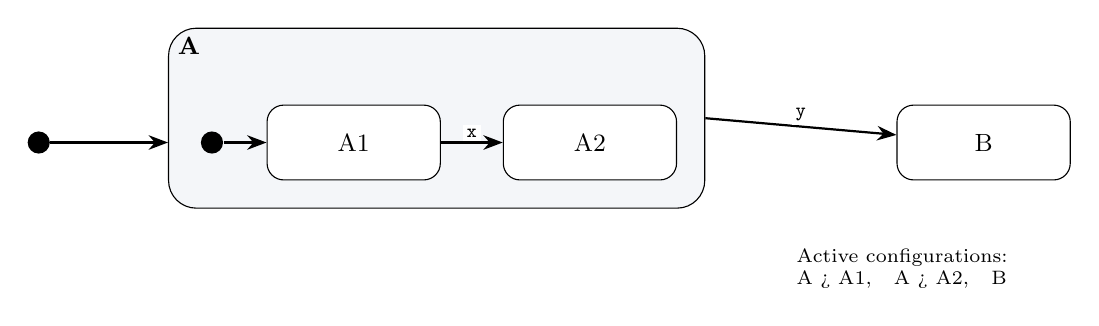
\begin{tikzpicture}
  \node[st] (a1) at (0,0) {A1};
  \node[st] (a2) at (3,0) {A2};
  \node[init] (ia) at (-1.8,0) {};
  \coordinate (t) at (-2,1.1);
  \begin{scope}[on background layer]\node[composite, fit=(a1)(a2)(ia)(t)] (A) {};\end{scope}
  \node[anchor=north west, font=\small\bfseries] at (A.north west) {A};
  \node[st] (b) at (8,0) {B};
  \node[init] (i0) at (-4,0) {};
  \draw[tr] (i0) -- (A.west |- i0);
  \draw[tr] (ia) -- (a1);
  \draw[tr] (a1) -- node[lbl, above]{x} (a2);
  \draw[tr] (A.east) -- node[lbl, above]{y} (b);
  \node[font=\scriptsize, align=left, anchor=west] at (5.5,-1.6) {Active configurations:\\ A > A1,\quad A > A2,\quad B};
\end{tikzpicture}
\caption{A composite state \code{A} with two substates. Event \code{y} leaves \code{A} from either
substate.}
\end{figure}

\section{Orthogonal regions}
\label{sec:regions}
A state can be divided into two or more \emph{regions}, drawn as dashed rectangles inside it. While
such an \emph{orthogonal state} is active, every one of its regions has exactly one active substate,
so the active configuration is a tree rather than a chain (Tutorial~5).
\begin{itemize}[itemsep=1pt]
  \item Each region needs its own initial pseudostate. Once a state has regions, all of its substates
        must lie inside one of them. A state with a single region behaves like an ordinary composite
        state.
  \item Entering the orthogonal state enters all of its regions, in diagram order. A transition that
        targets a substate of one region enters that region at the target and the other regions at
        their initial states, still in diagram order.
  \item An event is offered to every active region; several regions can handle the same event in one
        step. The orthogonal state itself only sees the event if none of its regions handled it. Once a
        transition in one region has left the orthogonal state, the remaining regions are not asked,
        even if the transition entered the state again.
  \item A transition leaving the orthogonal state --- from the state itself, or from a substate of one
        region to a state outside --- exits all regions, last region first, before the state's own
        exit actions run.
  \item The orthogonal state \emph{completes} when every region has reached a final state; then its
        completion transitions can fire.
  \item Transitions between different regions of the same state are not allowed, regions cannot be the
        source or target of transitions, and history pseudostates cannot be used in a state with
        several regions (a state with a single region can have one, inside that region).
\end{itemize}

\section{Initial and final states}
An \emph{initial pseudostate} has exactly one outgoing transition, without event or guard, to a state
inside its region (possibly nested deeper). That transition may have actions, which run before the
default state is entered.

A \emph{final state} has no outgoing transitions and no children. Reaching a top-level final state
means the machine has finished (\code{IsFinished} becomes true). A final state inside a composite state
is an ordinary leaf; the transitions of its enclosing states remain active.

\section{Transitions}
\begin{figure}[H]
\centering
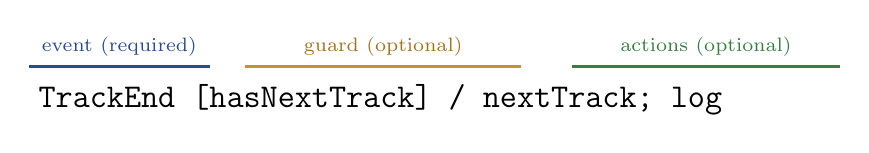
\begin{tikzpicture}
  \node[font=\ttfamily\large] (l) {TrackEnd [hasNextTrack] / nextTrack; log};
  \draw[thick, accent] ([yshift=3pt]l.north west) -- ++(2.3,0) node[midway, above, font=\scriptsize\rmfamily, text=accent]{event (required)};
  \draw[thick, gold] ($(l.north west)+(2.75,3pt)$) -- ++(3.5,0) node[midway, above, font=\scriptsize\rmfamily, text=gold!80!black]{guard (optional)};
  \draw[thick, tipframe] ($(l.north west)+(6.9,3pt)$) -- ++(3.4,0) node[midway, above, font=\scriptsize\rmfamily, text=tipframe]{actions (optional)};
\end{tikzpicture}
\caption{Anatomy of a transition label.}
\end{figure}
\begin{itemize}[itemsep=1pt]
  \item \textbf{Event} --- one of:
        \begin{itemize}[itemsep=0pt]
          \item an identifier; all such events form the \code{Event} enumeration;
          \item a timeout \code{after(}\textit{n}\,\code{ms}|\code{s}|\code{min)} (Section~\ref{sec:timeouts});
          \item empty, for a completion transition (Section~\ref{sec:completion}).
        \end{itemize}
  \item \textbf{Guard} --- the name of a Boolean method, optionally negated: \code{isReady},
        \code{!isBusy}. The transition fires only if the guard returns true.
  \item \textbf{Actions} --- method names separated by \code{;} or \code{,}, run in order.
\end{itemize}
A transition can start at a composite state; it then applies to all of its substates. A transition can
end at a composite state; the composite is then entered through its initial pseudostate. A self
transition exits and re-enters its state.

\begin{note}
Guards and actions are \emph{names}, not code. This keeps the diagram language-neutral and keeps your
logic in normal source files, where it can be debugged and unit-tested.
\end{note}

\section{Internal transitions}
An internal transition is a self transition that runs only its actions --- no exit actions, no entry
actions, and the active configuration does not change. On a composite state, the active substates stay
active. Create a self transition and tick \ui{Internal (no exit / entry)}; it is then listed inside the
state.

\begin{figure}[H]
\centering
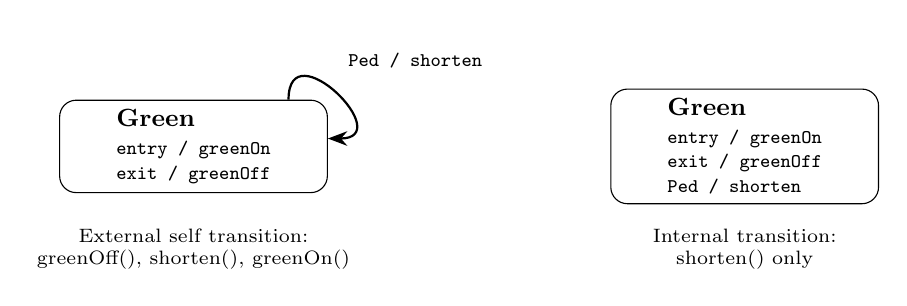
\begin{tikzpicture}
  \node[st, align=left, minimum width=3.4cm] (s1) at (0,0) {\textbf{Green}\\[-1pt]\scriptsize\ttfamily entry / greenOn\\[-2pt]\scriptsize\ttfamily exit / greenOff};
  \draw[tr] ($(s1.north east)+(-0.5,0)$) .. controls +(0,0.9) and +(0.9,0) .. ($(s1.east)+(0,0.1)$);
  \node[lbl, anchor=west] at ($(s1.north east)+(0.2,0.5)$) {Ped / shorten};
  \node[font=\scriptsize, align=center] at (0,-1.3) {External self transition:\\greenOff(), shorten(), greenOn()};
  \node[st, align=left, minimum width=3.4cm] (s2) at (7,0) {\textbf{Green}\\[-1pt]\scriptsize\ttfamily entry / greenOn\\[-2pt]\scriptsize\ttfamily exit / greenOff\\[-2pt]\scriptsize\ttfamily Ped / shorten};
  \node[font=\scriptsize, align=center] at (7,-1.3) {Internal transition:\\shorten() only};
\end{tikzpicture}
\caption{External self transition versus internal transition.}
\end{figure}

\section{History}
\label{sec:history}
A history pseudostate inside a composite state $C$ records the configuration of $C$ every time $C$ is
exited. A transition that targets the history pseudostate enters $C$ and restores it:
\begin{description}[style=nextline, itemsep=1pt]
  \item[Shallow history (H)] restores the last active \emph{direct} substate of $C$; if that substate is
    itself composite, it is entered through its initial pseudostate.
  \item[Deep history (H*)] restores the whole configuration below $C$: the last active substate at
    every level, entering every state on the way. Below an orthogonal state, every region is
    restored.
\end{description}
If $C$ has not been exited since \code{Start}, there is no history and $C$ is entered through its
initial pseudostate (\code{Start} forgets all history). Transitions that target $C$ itself always use
the initial pseudostate.

\begin{figure}[H]
\centering
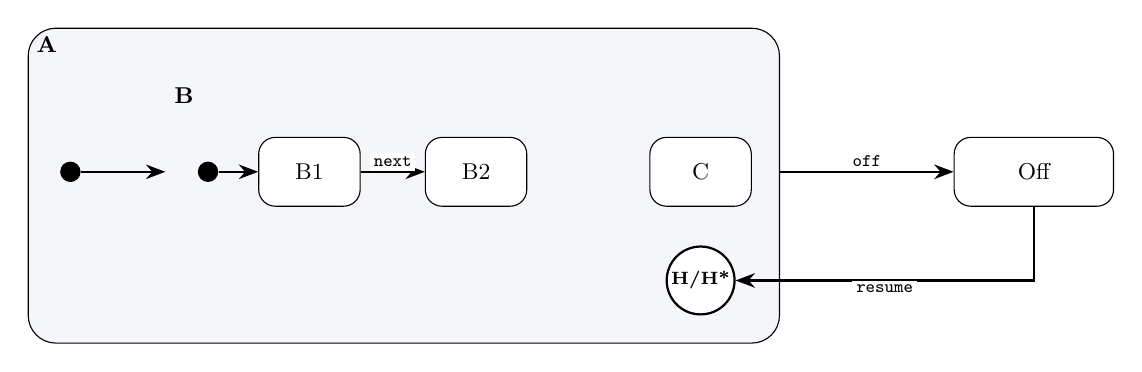
\begin{tikzpicture}[scale=0.92, every node/.style={transform shape}]
  \node[st, minimum width=1.4cm] (b1) at (0,0) {B1};
  \node[st, minimum width=1.4cm] (b2) at (2.3,0) {B2};
  \node[init] (ib) at (-1.4,0) {};
  \coordinate (bt) at (-1.6,0.9);
  \begin{scope}[on background layer]\node[composite, fit=(b1)(b2)(ib)(bt), fill=gold!10] (B) {};\end{scope}
  \node[anchor=north west, font=\small\bfseries] at (B.north west) {B};
  \node[st, minimum width=1.4cm] (c) at (5.4,0) {C};
  \node[init] (ia) at (-3.3,0) {};
  \node[hist] (h) at (5.4,-1.5) {H/H*};
  \coordinate (at) at (-3.5,1.6);
  \begin{scope}[on background layer]\node[composite, fit=(B)(c)(ia)(at)(h)] (A) {};\end{scope}
  \node[anchor=north west, font=\small\bfseries] at (A.north west) {A};
  \node[st] (off) at (10,0) {Off};
  \draw[tr] (ia) -- (B.west |- ia);
  \draw[tr] (ib) -- (b1);
  \draw[tr] (b1) -- node[lbl, above]{next} (b2);
  \draw[tr] (A.east |- off) -- node[lbl, above]{off} (off);
  \draw[tr] (off) |- node[lbl, pos=0.75, below]{resume} (h);
\end{tikzpicture}
\caption{Leave \code{A} from \code{B2} with \code{off}, then \code{resume}: shallow history restores
\code{B} and enters \code{B1} (its default); deep history restores \code{B2}.}
\end{figure}

A composite state can have at most one history pseudostate, and history pseudostates cannot have
outgoing transitions. A state with several orthogonal regions cannot have one; a state with a single
explicit region can, placed inside that region.

\section{Completion transitions}
\label{sec:completion}
A transition without an event is a \emph{completion transition}. It fires automatically when its source
state \emph{completes}:
\begin{itemize}[itemsep=1pt]
  \item a simple state completes as soon as it has been entered (after its entry actions);
  \item a composite state completes when its region reaches a final state.
\end{itemize}
Completion transitions are processed before \code{Start} or \code{Dispatch} returns, before any queued
event. They may have guards; if no guard is true the completion is discarded and the state simply stays
active. Typical uses are initialisation states (\code{Boot} in Tutorial~4) and ``when finished,
continue'' for composite states.

Completion transitions that lead back to a state that completes again immediately would fire for
ever. A cycle made only of unguarded completion transitions is therefore reported as an error. A cycle
that contains a guard is allowed (it ends when the guard becomes false), but in the generated code it
keeps \code{Dispatch} busy for as long as the guard holds; the simulator's engine gives up after 1000
completion transitions in one step.

\begin{figure}[H]
\centering
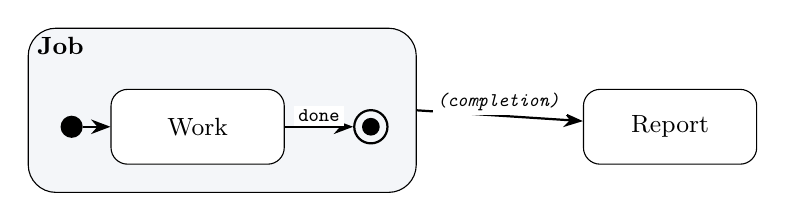
\begin{tikzpicture}
  \node[st] (w) at (0,0) {Work};
  \node[init] (iw) at (-1.6,0) {};
  \node[final] (f) at (2.2,0) {};
  \coordinate (t) at (-1.8,0.9);
  \begin{scope}[on background layer]\node[composite, fit=(w)(iw)(f)(t)] (J) {};\end{scope}
  \node[anchor=north west, font=\small\bfseries] at (J.north west) {Job};
  \node[st] (r) at (6,0) {Report};
  \draw[tr] (iw) -- (w);
  \draw[tr] (w) -- node[lbl, above]{done} (f);
  \draw[tr] (J.east) -- node[lbl, above]{\textit{(completion)}} (r);
\end{tikzpicture}
\caption{Reaching the final state completes \code{Job}; its event-less transition then fires.}
\end{figure}

\section{Timeouts}
\label{sec:timeouts}
An event written as \code{after(500ms)}, \code{after(2s)} or \code{after(1min)} (no unit means
milliseconds) is a \emph{timeout}. Each distinct timeout of a state becomes an event with a generated
name, \textit{State}\code{\_After}\textit{n}\code{ms}, e.g. \code{Collecting\_After30000ms}. The
generated class calls two hooks that you implement with your platform's timers:
\begin{itemize}[itemsep=1pt]
  \item \code{StartTimer(timeout, milliseconds, generation)} after the state has been entered (after
        its entry actions);
  \item \code{CancelTimer(timeout)} when the state is exited (before its exit actions).
\end{itemize}
When a timer elapses, call \code{DispatchTimeout(timeout, generation)} with the generation number that
\code{StartTimer} received. Every start of a timer gets a new generation, and the call is ignored
(returning \code{false}) if that timer has been cancelled or restarted since. A late timer is
therefore harmless even when its state has been left and re-entered in the meantime --- it cannot
cut the new waiting time short. A timer fires once: after its timeout has been dispatched, a repeated
call with the same generation is ignored too, even if the timeout's guard was false or its transition
internal. An external self transition restarts the timer; an internal transition does not. Timeouts
can have guards and actions like any other transition.

\section{Choice points}
\label{sec:choice}
A choice point (diamond) splits a transition into alternative branches. The incoming transition
carries the event (and optionally a guard and actions); each outgoing branch carries a guard and
optionally actions. One branch may have the guard \code{else} (or no guard), which is taken when no
other guard is true. Branches can lead to states, history pseudostates or further choice points.

\begin{figure}[H]
\centering
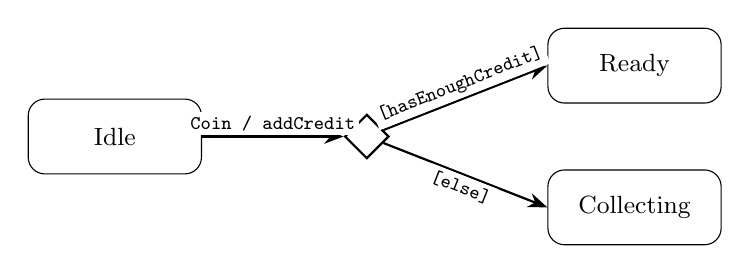
\begin{tikzpicture}
  \node[st] (i) at (0,0) {Idle};
  \node[choicept] (c) at (3.2,0) {};
  \node[st] (r) at (6.6,0.9) {Ready};
  \node[st] (k) at (6.6,-0.9) {Collecting};
  \draw[tr] (i) -- node[lbl, above]{Coin / addCredit} (c);
  \draw[tr] (c) -- node[lbl, above, sloped]{[hasEnoughCredit]} (r.west);
  \draw[tr] (c) -- node[lbl, below, sloped]{[else]} (k.west);
\end{tikzpicture}
\caption{A choice point with an \code{[else]} branch.}
\end{figure}

MachinaState evaluates all guards on the path \emph{before} the transition starts: first the guard of
the incoming transition, then the branch guards in order (\code{else} last). Only when a complete path
is found does it exit the source states, run the actions of all segments (incoming first), and enter
the target. If no branch is enabled, nothing happens and the transition counts as not enabled, so the
event continues to the next candidate (an outer state, for example). In UML terms this is the
semantics of a \emph{junction}; it guarantees that a transition never stops half-way.

Consequently a branch guard cannot see the effect of the incoming transition's actions --- in
Tutorial~4, \code{hasEnoughCredit} adds the incoming coin to the credit itself. Branch guards and actions
receive the parameters of the triggering event.

\section{Event parameters}
\label{sec:params}
Declare parameters per event with nothing selected, as a comma-separated list such as
\code{int level} or \code{const std::string\& name, int retries}. Each entry must be written as
\code{type name}; default values are ignored. The parameters are passed to the guards and actions of
every transition triggered by that event. Consequently:
\begin{itemize}[itemsep=1pt]
  \item a hook used with several events must receive the same parameter list everywhere;
  \item entry, exit and initial actions never receive parameters.
\end{itemize}
In the generated code, each event with parameters gets a typed dispatch method, for example
\code{DispatchVolume(int level)}.

\section{Supported and unsupported UML features}
\begin{center}
\renewcommand{\arraystretch}{1.15}
\begin{tabularx}{\linewidth}{@{}>{\raggedright\arraybackslash}p{0.57\linewidth}>{\raggedright\arraybackslash}X@{}}
\toprule
\textbf{UML feature} & \textbf{Status} \\
\midrule
Simple and composite states, arbitrary nesting & supported \\
Initial, final, shallow and deep history pseudostates & supported \\
Entry and exit actions, transition actions & supported \\
Guards (single, optionally negated, method name) & supported \\
Internal transitions & supported \\
Event parameters & supported \\
Completion (event-less) transitions & supported \\
Time events (\code{after}) & supported, through timer hooks \\
Choice pseudostates & supported, guards evaluated before the transition starts (junction semantics) \\
Orthogonal (parallel) regions & supported, without history in orthogonal states \\
Time events (\code{at}), \code{do} activities, deferred events & not supported \\
\bottomrule
\end{tabularx}
\end{center}

%=====================================================================
\chapter{Execution Semantics}
\label{ch:semantics}

All six generated variants (C++, C\# and C, each switch-based and table-based) and the simulator
implement exactly the semantics in this chapter. The simulator runs a reference engine, and the test
suite checks that it and all generated variants produce identical traces.

\section{Starting}
\code{Start()} first resets the machine: it cancels every running timer (calling \code{CancelTimer},
and giving it a new generation so that a \code{DispatchTimeout} still on its way is ignored), forgets
all history, discards pending completions and queued events, and sets the active state to
\emph{none}. Start is a reset, not a transition: states that were active before are not exited, so their
exit actions do not run. Then it runs the actions of the top-level initial transition and enters its
target. Entering a composite state continues with its initial transition, until a leaf state is
reached; entering an orthogonal state enters each of its regions in turn. Completion transitions and
queued events are then processed exactly as after a dispatched event.

\section{Dispatching an event}
\label{sec:dispatch}
\code{Dispatch} processes one event \emph{to completion} before returning:

\begin{lstlisting}[language=C++, caption={Dispatch algorithm (pseudocode).}]
handled = false
for (s = innermost active state; s != none && !handled; s = parent(s))
    for (t in transitions leaving s for this event,
              those that may not fire first, in diagram order)
        if (guard(t) holds && (t has no choice point || a branch path is enabled))
            fire(t); handled = true; break
if (handled)
    while (a state has completed)        // run to completion
        fire its enabled completion transition, if any
drain the event queue (each queued event is dispatched like this one)
return handled
\end{lstlisting}

Inner states therefore take priority over outer ones, and within a state guarded transitions are
checked before the unguarded one (Figure~\ref{fig:priority}). With orthogonal regions, ``the innermost
active state'' is one state per region: the event is offered to each active region in diagram order
(each region applying the loop above), and bubbles up to the orthogonal state only if no region handled
it. If a transition in one region leaves the orthogonal state, the remaining regions are not asked
--- even when the transition enters the orthogonal state again (a self transition of the orthogonal
state, for example), so that its freshly entered regions do not see the same event a second time.

\begin{figure}[H]
\centering
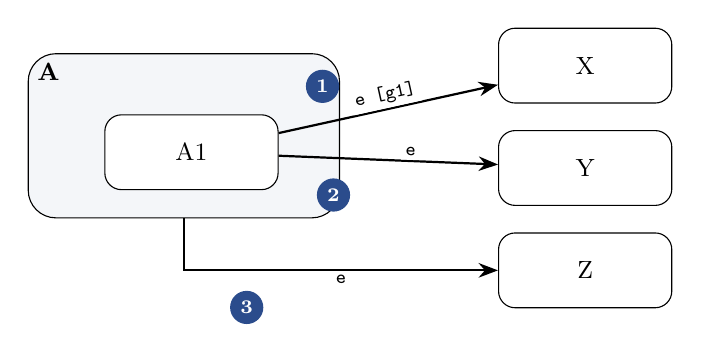
\begin{tikzpicture}
  \node[st] (a1) at (0,0) {A1};
  \coordinate (t) at (-1.3,0.9);
  \begin{scope}[on background layer]\node[composite, fit=(a1)(t), inner xsep=22pt] (A) {};\end{scope}
  \node[anchor=north west, font=\small\bfseries] at (A.north west) {A};
  \node[st] (x) at (5,1.1) {X};
  \node[st] (y) at (5,-0.2) {Y};
  \node[st] (z) at (5,-1.5) {Z};
  \draw[tr] (a1) -- node[lbl, above, sloped]{e [g1]} node[stepno, pos=0.2, above=7pt]{1} (x);
  \draw[tr] (a1) -- node[lbl, above, sloped, pos=0.6]{e} node[stepno, pos=0.25, below=7pt]{2} (y);
  \draw[tr] (A.south) |- node[lbl, pos=0.75, below]{e} node[stepno, pos=0.6, below=7pt]{3} (z);
\end{tikzpicture}
\caption{Evaluation order for event \code{e} while \code{A1} is active: \code{A1}'s guarded transition,
then \code{A1}'s unguarded one. \code{A}'s transition \textcircled{\scriptsize 3} is only considered
if \code{A1} has no enabled transition for \code{e}.}
\label{fig:priority}
\end{figure}

\section{Firing a transition}
For an external transition from source $S$ to target $T$:
\begin{enumerate}[itemsep=1pt]
  \item Determine the \emph{least common ancestor} (LCA): the innermost state that strictly contains
        both $S$ and $T$, or the top level.
  \item Exit all active states below the LCA, innermost first, running exit actions (and recording
        history of composite states being exited).
  \item Run the transition's actions.
  \item Enter the states from below the LCA down to $T$, outermost first, running entry actions.
  \item While the entered state is composite, follow its initial transition (running its actions).
\end{enumerate}
An internal transition only runs its actions. A transition to a history pseudostate of $C$ uses $C$ as
the target for the LCA, but restores the recorded configuration of $C$ if there is one
(Section~\ref{sec:history}). A transition through choice
points first selects a complete path (Section~\ref{sec:choice}), then performs steps 1--5 with the
final target and the actions of all segments in order. Exiting a state with timeouts cancels its
timers; entering it starts them. Entering a leaf state that has completion transitions --- or a final
state whose parent has them --- marks that state as completed.

\begin{figure}[H]
\centering
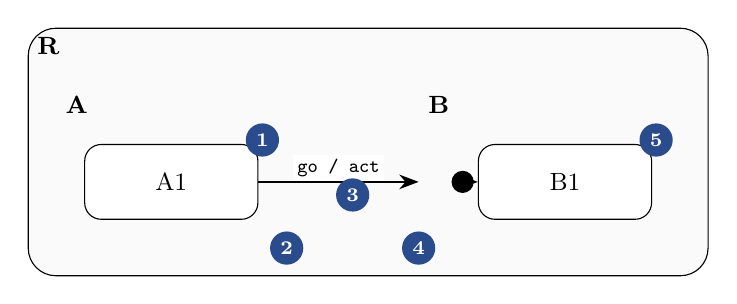
\begin{tikzpicture}
  \node[st] (a1) at (0,0) {A1};
  \coordinate (at) at (-0.8,0.85);
  \begin{scope}[on background layer]\node[composite, fit=(a1)(at)] (A) {};\end{scope}
  \node[anchor=north west, font=\small\bfseries] at (A.north west) {A};
  \node[st] (b1) at (5,0) {B1};
  \node[init] (ib) at (3.7,0) {};
  \coordinate (bt) at (3.5,0.85);
  \begin{scope}[on background layer]\node[composite, fit=(b1)(ib)(bt)] (B) {};\end{scope}
  \node[anchor=north west, font=\small\bfseries] at (B.north west) {B};
  \coordinate (rt) at (-1.2,1.6);
  \begin{scope}[on background layer]\node[composite, fit=(A)(B)(rt), fill=black!2] (R) {};\end{scope}
  \node[anchor=north west, font=\small\bfseries] at (R.north west) {R};
  \draw[tr] (ib) -- (b1);
  \draw[tr] (a1.east) -- node[lbl, above]{go / act} (B.west |- a1.east);
  \node[stepno] at ($(a1.north east)+(0.05,0.05)$) {1};
  \node[stepno] at (A.south east) {2};
  \node[stepno] at ($(A.east)!0.5!(B.west)+(0,-0.35)$) {3};
  \node[stepno] at (B.south west) {4};
  \node[stepno] at ($(b1.north east)+(0.05,0.05)$) {5};
\end{tikzpicture}
\caption{Transition \code{go / act} from \code{A1} to \code{B}. The LCA is \code{R}, so the order is:
\textcircled{\scriptsize 1} exit \code{A1}, \textcircled{\scriptsize 2} exit \code{A},
\textcircled{\scriptsize 3} \code{act()}, \textcircled{\scriptsize 4} enter \code{B},
\textcircled{\scriptsize 5} enter \code{B1} via \code{B}'s initial transition. \code{R} stays active.}
\end{figure}

\section{Orthogonal regions}
For a state $O$ with regions $R_1,\dots,R_n$:
\begin{itemize}[itemsep=1pt]
  \item \textbf{Entering} $O$ runs its entry actions, then enters $R_1,\dots,R_n$ in order. A region
        that contains the transition's target is entered along the path to the target; every other
        region follows its initial transition. The order does not depend on where the target is: with
        a target in $R_2$, $R_1$ is entered (by default) before $R_2$.
  \item \textbf{Dispatching} offers the event to $R_1,\dots,R_n$ in order and stops as soon as a
        transition taken in one region has exited $O$, whether or not it re-entered $O$.
  \item \textbf{Exiting} $O$ exits $R_n,\dots,R_1$ in reverse order --- each one innermost state
        first --- then cancels $O$'s timers and runs its exit actions.
  \item A final state reached in a region marks $O$ as \textbf{completed} once every region's active
        state is final. The completion is processed after the current step, like any other.
\end{itemize}

\section{Worked example}
The table traces the hierarchical traffic light from Tutorial~2 (compare with the program output in
Section~7 of that tutorial).

\begin{center}
\small
\begin{tabularx}{\linewidth}{@{}llX@{}}
\toprule
\textbf{Event} & \textbf{Active before} & \textbf{Effect} \\
\midrule
\code{Start()}            & ---                  & enter \code{Off} \\
\code{PowerOn}            & \code{Off}           & exit \code{Off}; enter \code{Operating}; enter \code{Red}, \code{redOn()} \\
\code{Timer}              & \code{Operating>Red} & handled by \code{Red}: exit \code{Red}, \code{redOff()}; enter \code{Green}, \code{greenOn()} \\
\code{PedestrianRequest}  & \code{Operating>Green} & internal: \code{shortenGreen()} \\
\code{Fault}              & \code{Operating>Green} & not handled by \code{Green}, bubbles to \code{Operating}: exit \code{Green}, \code{greenOff()}; exit \code{Operating} (history := \code{Green}); \code{logFault()}; enter \code{Flashing}, \code{flashOn()} \\
\code{Repair}             & \code{Flashing}      & exit \code{Flashing}, \code{flashOff()}; enter \code{Operating}; resume \code{Green}, \code{greenOn()} \\
\code{Timer}              & \code{Operating>Green} & exit \code{Green}; enter \code{Yellow} \\
\bottomrule
\end{tabularx}
\end{center}

\section{Rules for hooks}
Guards and actions run \emph{during} \code{Dispatch}. They must not call \code{Dispatch} (or
\code{Start}) recursively: the machine is in the middle of a transition. If an action needs to raise a
follow-up event, enable \ui{Queue} and call \code{Post} (Section~\ref{sec:queue}).
Guards should be free of side effects; they may be evaluated without their transition firing.

%=====================================================================
\chapter{Simulator}
\label{ch:sim}

Click \ui{Simulate} to start. The simulator runs the diagram on the same reference engine that the
test suite compares with every generated variant, so a step in the simulator does exactly what
\code{Dispatch} does in the generated code: choice points, completion transitions and queued events
are all processed within the step. The machine is started, editing is disabled and the side panel
changes to the simulation view:

\begin{description}[style=nextline, itemsep=2pt]
  \item[Active] the active leaf states with their ancestors, e.g. \code{Operating > Green}; with
    orthogonal regions one path per region, separated by \code{|}. ``State machine finished'' appears
    once a top-level final state is reached.
  \item[Reset / Record / Stop] restart the machine, start recording a scenario, or leave the simulator.
  \item[Events] one button per event. Events that no active state handles right now are shown dimmed;
    firing one is still allowed and logs that it was ignored. Events with parameters have an argument
    field: enter the values separated by commas (numbers, \code{true}/\code{false}, or text).
  \item[Running timers] one button per running timer, e.g. \ui{after 2 s in Dropping}. Clicking it lets
    the timer elapse, like \code{DispatchTimeout} with the current generation. The timer then
    disappears from the list (timers are one-shot) unless the transition re-enters its state and
    restarts it.
  \item[Guard results] one check box per guard. The simulator cannot run your code, so you decide what
    each guard returns; a ticked box means \code{true}. Negated guards (\code{!isBusy}) use the same box.
    The trace shows each guard call with its arguments and result.
  \item[Scenarios] the scenarios saved in the diagram, with \ui{Run}, \ui{Step} and \ui{\texttimes}
    (delete) (Section~\ref{sec:scenarios}).
  \item[Coverage] how many transitions and choice branches have been taken since the simulator was
    started, out of all that can be taken (initial transitions are not counted). \ui{Highlight untaken}
    draws the others dashed and in red, also when they have their own colour; \ui{Clear} resets the
    count.
  \item[Trace] every event, transition, exit, action (with arguments) and entry in execution order ---
    the same lines the generated \code{Trace} hook reports.
\end{description}

Active states are drawn in green and the transitions taken in the last step are highlighted. Pan and
zoom remain available while simulating. If the diagram has errors, the panel lists them instead.
If completion transitions keep firing without settling (more than 1000 in one step, see
Section~\ref{sec:completion}), the simulator stops, reports a probable endless loop in the trace and
refuses further events until \ui{Reset}.

\section{Scenarios}
\label{sec:scenarios}
A \emph{scenario} is a named sequence of steps saved in the diagram. Each step is an event, with its
arguments and the guards that were \emph{false} when it was fired.
\begin{itemize}[itemsep=1pt]
  \item \ui{Record} restarts the simulation and records every event you fire. \ui{Save (\textit{n})}
        stores the recording as \code{Scenario \textit{n}}; \ui{Discard} drops it.
  \item \ui{Run} restarts the simulation and replays all steps, setting the guard results recorded for
        each step. \ui{Step} restarts it and replays one step per click.
  \item The name field renames a scenario; \ui{\texttimes} deletes it. Both are document edits and can
        be undone.
\end{itemize}
Because a replay sets the guard results itself, a scenario always takes the same path through an
unchanged diagram. After a change, replaying the scenarios and comparing the trace is a quick
regression test; a step that is now ignored shows up as \code{ignored} in the trace. A replayed
timeout whose timer is not running at that point (its state was left, or the timer already elapsed) is
not dispatched; the trace marks it as a stale timeout.

\begin{tip}
Use the simulator as an executable specification: walk through each requirement and compare the
trace with what you expect. A trace that is surprising in the simulator will be equally surprising in
the generated code.
\end{tip}

%=====================================================================
\chapter{Code Generation}
\label{ch:codegen}

\section{Generating}
Choose language, style and options in the toolbar and click \ui{Generate Code}. Alternatively run
\ui{MachinaState: Generate State Machine Code} from the Command Palette, the editor title bar or the
context menu of a \code{.machina} file in the Explorer; these use the language and style stored in
the diagram and ask only if none are stored. The file \code{<ClassName>.hpp} or \code{<ClassName>.cs}
--- for C the pair \code{<ClassName>.h} and \code{<ClassName>.c} --- is written next to the diagram
(overwriting a previous version) and opened beside the editor. A diagram that has never been saved asks
for an output folder instead, and confirms before overwriting existing files.

\begin{caution}
Never edit the generated file --- it is overwritten on every generation. Put your code in a subclass.
Generated files can be checked into version control or generated as part of your build.
\end{caution}

\section{Generated interface}
\begin{longtable}{@{}p{4.4cm}p{10cm}@{}}
\toprule
\textbf{Member} & \textbf{Description} \\
\midrule
\endhead
\code{enum State}             & All states in pre-order (parents before children), plus \code{None}. \\
\code{enum Event}             & All events used by transitions. \\
\code{Start()}                & Resets the machine (cancels running timers, forgets history) and enters the initial configuration through the top-level initial transition. \\
\code{Dispatch(Event)}        & Processes one event; returns \code{true} if a transition fired. Events with parameters are rejected (\code{false}). \\
\code{Dispatch\textit{Event}(\dots)} & Typed method per event with parameters, e.g. \code{DispatchEnterCode(int code)}. \\
\code{Completion} event       & Present when the diagram has completion transitions; used internally and rejected by \code{Dispatch}. \\
\textit{State}\code{\_After}\textit{n}\code{ms} events & One per timeout, reported by \code{StartTimer}. \\
\code{DispatchTimeout(Event, generation)} & Generated with timeouts; call it when a timer elapses (Section~\ref{sec:timers}). Each timer fires at most once per start. \\
\code{Current}                & Innermost active state, following the first region of orthogonal states (method in C++, property in C\#). \\
\code{IsIn(State)}            & True if the state is active, also as an ancestor of an active state or in any region. \\
\code{IsFinished}             & True when a top-level final state is active (method in C++, property in C\#). \\
\code{ParentOf(State)}        & Static; the enclosing state or \code{None}. \\
\code{StateName}, \code{EventName} & Static, C++ only; use \code{ToString()} in C\#. \\
\code{kStateCount}, \code{kEventCount} & C++ only; number of states and events. \\
Guards and actions            & Pure virtual (C++) / \code{protected abstract} (C\#) hooks. \\
\code{Trace(TraceKind, name)} & Optional, virtual with empty default (Section~\ref{sec:trace}). \\
\code{Lock()}, \code{Unlock()} & Optional, abstract (Section~\ref{sec:threads}). \\
\code{StartTimer}, \code{CancelTimer} & Abstract; generated when the diagram has timeouts (Section~\ref{sec:timers}). \\
\code{Post(Event)}, \code{Post\textit{Event}(\dots)} & Optional, protected; queue an event from a hook (Section~\ref{sec:queue}). \\
\code{kQueueCapacity}         & With \ui{Queue}; size of the queue (\code{codegen.queueCapacity}, default 16). \code{QueueCapacity} in C\#, \code{\dots\_QueueCapacity} in C. \\
\bottomrule
\end{longtable}

\section{Switch-based versus table-based}
\label{sec:styles}
Both styles have the same interface and identical behaviour.

\begin{center}
\begin{tabularx}{\linewidth}{@{}lXX@{}}
\toprule
 & \textbf{Switch-based} & \textbf{Table-based} \\
\midrule
Event handling & Nested \code{switch} over state and event & Loop over a constant transition table \\
Hierarchy      & \code{ParentOf} as a \code{switch} & Parent lookup array \\
Entry/exit     & \code{switch} in \code{OnEntry}/\code{OnExit} & Arrays of member-function pointers (C++) or delegates (C\#) \\
Code size      & Grows with the number of transitions & Mostly data; small fixed code \\
Debugging      & Step through readable control flow & Inspect table rows \\
Best for       & Small to medium machines, readability & Large machines, data-driven inspection \\
\bottomrule
\end{tabularx}
\end{center}

\lstinputlisting[language=C++, caption={Switch-based: event handling for the flat traffic
light.}]{generated/snippets/switch-handle.hpp}

\lstinputlisting[language=C++, caption={Table-based: the same transitions as
data.}]{generated/snippets/table-rows.hpp}

\section{C++ specifics}
\begin{itemize}[itemsep=1pt]
  \item Single self-contained header, C++17 (uses \code{inline} variables for the tables). No heap
        allocation, no exceptions, no RTTI --- suitable for embedded targets.
  \item Hooks are pure virtual member functions; derive and \code{override} them.
  \item Event arguments are passed through a pointer to a stack-allocated argument struct that is
        valid only during the call, so reference parameters such as \code{const std::string\&} are
        never copied.
  \item Namespaces written with dots are converted to nested C++ namespaces.
\end{itemize}

\section{C specifics}
\label{sec:c}
The C target generates a header and a source file in C99, for compilers and code bases that cannot
use C++. Everything is prefixed with the namespace and class name (\code{Demo\_TrafficLight\_\dots})
to avoid clashes.
\begin{itemize}[itemsep=1pt]
  \item The machine is a plain \code{struct} that you allocate (statically, on the stack or inside your
        own structure); the generated code never allocates memory. Treat its members as private.
  \item Guards, actions and the optional services (\code{Trace}, \code{Lock}/\code{Unlock},
        \code{StartTimer}/\code{CancelTimer}) are function pointers in a \code{\dots\_Hooks} structure.
        Each receives the \code{void* context} passed to \code{\dots\_Init}, followed by the event
        parameters. All members must be set, except \code{Trace}, which may be \code{NULL}.
  \item The public functions mirror the C++ interface: \code{\dots\_Init}, \code{\dots\_Start},
        \code{\dots\_Dispatch}, \code{\dots\_Dispatch\textit{Event}(machine, args\dots)},
        \code{\dots\_DispatchTimeout}, \code{\dots\_Current}, \code{\dots\_IsIn},
        \code{\dots\_IsFinished}, \code{\dots\_ParentOf}, \code{\dots\_StateName},
        \code{\dots\_EventName}. With \ui{Queue}, hooks can call \code{\dots\_Post} and the typed
        \code{\dots\_Post\textit{Event}} functions; the queue is a fixed array of
        \code{codegen.queueCapacity} entries.
  \item Switch-based and table-based styles are available as in C++; the table-based variant uses
        constant arrays of function pointers.
\end{itemize}
The traffic light of Tutorial~1, generated as C with \ui{Trace}, is driven like this:

\lstinputlisting[language=C, caption={\code{traffic\_flat.c}, compiled with
\code{gcc -std=c99 -Wall -Wextra -Werror -pedantic} together with the generated
\code{TrafficLight.c}.}]{examples/traffic_flat.c}

\lstinputlisting[style=output, caption={Output of the C program.}]{generated/traffic_flat_c.txt}

The generated header is listed in Appendix~\ref{app:c}.

\section{C\# specifics}
\begin{itemize}[itemsep=1pt]
  \item The class is \code{public abstract} and uses nullable annotations (\code{\#nullable enable}).
  \item Hooks are \code{protected abstract} methods; \code{Trace} is \code{protected virtual}.
  \item Event arguments are stored in private fields before dispatch.
  \item Table-based code builds its tables in the protected constructor using method groups and lambdas.
\end{itemize}

\section{Tracing}
\label{sec:trace}
With \ui{Trace} ticked, the class gets a \code{TraceKind} enumeration and a virtual
\code{Trace(TraceKind kind, name)} method that does nothing by default:
\begin{center}
\begin{tabularx}{\linewidth}{@{}lX@{}}
\toprule
\textbf{Kind} & \textbf{Reported when / name} \\
\midrule
\code{Start}      & \code{Start()} is called; the class name. \\
\code{Event}      & \code{Dispatch} receives an event; the event name. \\
\code{Ignored}    & No state handled the event; the event name. \\
\code{Transition} & A transition fires, before any exit: \code{"S -> T"}, \code{"S (internal)"} or \code{"S -> T (history)"}. \\
\code{Exit}       & A state is about to be exited (before its exit actions). \\
\code{Enter}      & A state has been entered (before its entry actions). \\
\bottomrule
\end{tabularx}
\end{center}
In C++ the names are string literals (no allocation). Tutorials 2 and 3 show complete examples.

\section{Thread safety}
\label{sec:threads}
By default the machine is not thread-safe. With \ui{Thread-safe} ticked, the class declares two hooks
that you implement with any synchronisation primitive (mutex, critical section, RTOS semaphore,
interrupt masking):
\begin{center}
\begin{tabularx}{\linewidth}{@{}lX@{}}
\toprule
C++  & \code{virtual void Lock() const = 0;}\quad\code{virtual void Unlock() const = 0;} \\
C\#  & \code{protected abstract void Lock();}\quad\code{protected abstract void Unlock();} \\
\bottomrule
\end{tabularx}
\end{center}
\code{Start}, \code{Dispatch}, the typed dispatch methods, \code{DispatchTimeout}, \code{Current},
\code{IsIn} and \code{IsFinished} acquire the lock on entry and release it on exit, also when an
exception is thrown (RAII guard in C++, \code{try}/\code{finally} in C\#). Hooks therefore run while
the lock is held. \code{Post}, the static members (\code{ParentOf}, \code{StateName},
\code{EventName}) and, in C, \code{\dots\_Init} do not lock.

\begin{lstlisting}[language=C++]
class Player : public Demo::MediaPlayer {
  protected:
    void Lock() const override   { mutex_.lock(); }
    void Unlock() const override { mutex_.unlock(); }
  private:
    mutable std::mutex mutex_;     // const hooks need a mutable mutex
};
\end{lstlisting}

\begin{caution}
Hooks must not call public members of the machine (\code{IsIn}, \code{Current}, \dots) unless the lock
is re-entrant (\code{std::recursive\_mutex}; \code{Monitor} in C\# already is). Never call
\code{Dispatch} from a hook, even with a re-entrant lock.
\end{caution}

\section{Event queue}
\label{sec:queue}
Actions often need to raise further events --- ``credit limit exceeded, cancel'', ``self-test failed,
enter error mode''. Calling \code{Dispatch} from a hook is not allowed, because the machine is in the
middle of a transition. With \ui{Queue} ticked, the class instead offers protected \code{Post} methods:
\begin{lstlisting}[language=C++]
bool Post(Event event);               // events without parameters
bool PostCoin(int cents);             // one typed method per event with parameters
\end{lstlisting}
A posted event is stored and dispatched after the current \code{Start}/\code{Dispatch} call has
finished its transition and all completion transitions --- still inside the same call, before it
returns. Events posted while the queue is being drained are appended and processed in order.
\begin{itemize}[itemsep=1pt]
  \item In C++ the queue is a ring buffer of \code{kQueueCapacity} entries inside the object (no heap),
        and in C a ring buffer of \code{\dots\_QueueCapacity} entries inside the machine structure.
        Parameters are copied by value: a reference and a top-level \code{const} are removed from the
        declared type (\code{const std::string\&} is stored as \code{std::string}, \code{const int}
        as \code{int}), but a pointer is stored as it is (\code{const char*}), so what it points to
        must outlive the queued event.
  \item In C\# the queue holds at most \code{QueueCapacity} events; the closure stored for a typed
        \code{Post\textit{Event}} captures its arguments.
  \item \code{Post} returns \code{false} when the queue is full, and for events that cannot be posted
        (\code{Completion}, or an event with parameters passed to the untyped \code{Post}).
  \item \code{Post} does not lock; it is meant to be called from hooks, which already run under the
        lock when \ui{Thread-safe} is enabled. From other threads, call \code{Dispatch}.
\end{itemize}
Tutorial~4 shows \code{Post} in action.

\section{Timers}
\label{sec:timers}
For diagrams with \code{after(...)} transitions the class declares
\begin{lstlisting}[language=C++]
virtual void StartTimer(Event timeout, unsigned milliseconds, unsigned generation) = 0;   // C++
virtual void CancelTimer(Event timeout) = 0;
\end{lstlisting}
(in C\# the same as \code{protected abstract} methods with \code{int} parameters; in C as
\code{StartTimer} and \code{CancelTimer} members of the hooks structure). Implement them with whatever
timer your platform offers. When a timer elapses, pass the event and the generation it was started
with to \code{DispatchTimeout}:

\lstinputlisting[language=C++, caption={\code{DispatchTimeout} in the generated vending
machine.}]{generated/snippets/vending-timers.hpp}

Each timeout event has a generation counter that is incremented whenever its timer is started, and an
\emph{armed} flag that is cleared when the timer is cancelled or has fired, i.e.\ as soon as its
timeout is dispatched: a timer fires at most once per start, even if the timeout's guard is false or
its transition is internal. A timeout that arrives after its state was left, after the state was left
and entered again, or a second time for the same start, does not match and is ignored --- even if
your timer implementation cannot cancel a callback that is already on its way. \code{Start} cancels
every running timer (through \code{CancelTimer}) and makes outstanding timeouts stale.

Calling \code{Dispatch(timeout)} (or \code{Post(timeout)}) directly is still possible, for example
to drive timeouts by hand in a test: it skips the generation check, but disarms the timer like
\code{DispatchTimeout} does, so the timer's own callback is ignored when it arrives later. In C\#:
\begin{lstlisting}[language={[Sharp]C}]
private readonly Dictionary<Event, Timer> timers = new();

protected override void StartTimer(Event timeout, int milliseconds, int generation) =>
    timers[timeout] = new Timer(_ => DispatchTimeout(timeout, generation), null, milliseconds, Timeout.Infinite);

protected override void CancelTimer(Event timeout)
{
    if (timers.Remove(timeout, out var timer))
        timer.Dispose();
}
\end{lstlisting}
The timer callback runs on a thread-pool thread, so combine this with \ui{Thread-safe}. On embedded
systems, record the deadline in \code{StartTimer}, check it in the main loop or a timer interrupt, and
call \code{DispatchTimeout} from the main loop.

\section{Integration patterns}

\subsection{Unit testing}
Because all hooks are virtual, a test double can record calls and control guards:
\begin{lstlisting}[language=C++]
struct TestLight : Demo::TrafficLight {
    std::vector<std::string> calls;
    void redOn() override     { calls.push_back("redOn"); }
    void redOff() override    { calls.push_back("redOff"); }
    void greenOn() override   { calls.push_back("greenOn"); }
    void greenOff() override  { calls.push_back("greenOff"); }
    void yellowOn() override  { calls.push_back("yellowOn"); }
    void yellowOff() override { calls.push_back("yellowOff"); }
};

TEST(TrafficLight, TimerAdvancesFromRedToGreen) {
    TestLight light;
    light.Start();
    ASSERT_EQ(light.Current(), TestLight::State::Red);
    EXPECT_TRUE(light.Dispatch(TestLight::Event::Timer));
    EXPECT_EQ(light.Current(), TestLight::State::Green);
    EXPECT_EQ(light.calls, (std::vector<std::string>{ "redOn", "redOff", "greenOn" }));
}
\end{lstlisting}

%=====================================================================
\chapter{Import and Export}
\label{ch:interop}

MachinaState reads and writes three textual formats, so that diagrams can move to and from other tools
and into documentation. Export writes a file next to the diagram; import creates a new
\code{.machina} file, lays it out automatically (Section~\ref{sec:layout}) and opens it. Problems
found during import are reported as warnings; the elements concerned are skipped.

\section{PlantUML}
\ui{Export Diagram as PlantUML} writes a PlantUML state diagram that renders with any PlantUML
installation or documentation tool that embeds it. States, nesting, regions (separated by \code{--}),
initial and final states, history (\code{[H]}, \code{[H*]}), choice points (\code{<<choice>>}),
entry and exit actions, internal transitions and labels \code{event [guard] / action} are written in
PlantUML syntax. Details that PlantUML has no notation for --- the namespace, event parameters and
region names --- are kept in special comments, so an exported file imports back without loss.
This is the export of the washing machine of Tutorial~5:
\begin{lstlisting}
@startuml Washer
' @namespace Appliances
' @event SetTemp(int celsius)
state Idle
state Running {
  ' @region Program
  state Washing
  Washing : entry / motorSlow
  ...
  [*] --> Washing
  --
  ' @region Heater
  state Heating
  ...
}
Running : entry / lockDoor
Idle --> Running : Start / fillWater
Washing --> Rinsing : after(30s) / drain
Running --> Idle : / beep
@enduml
\end{lstlisting}
\ui{Import PlantUML, SCXML or Mermaid State Machine} reads the common subset of PlantUML's state diagram
syntax: \code{state} declarations with nested blocks, aliases (\code{state "Long name" as X}),
\code{[*]} for initial and final states, \code{<<choice>>}, \code{<<end>>}, \code{[H]} and
\code{[H*]}, \code{--} region separators, \code{X : entry / a} and \code{X : exit / b}, and transitions
with any arrow style (\code{->}, \code{-->}, \code{-up->}, \dots). It also reads internal transitions
written as description lines (\code{X : event [guard] / action}; an internal transition with neither
guard nor action is exported as \code{X : event /}). Notes, legends, skin parameters and other layout
commands are skipped silently; a note without its \code{end note} and other lines it does not
understand are reported and skipped.

\section{Mermaid}
\label{sec:mermaid}
Mermaid diagrams render directly in GitHub and GitLab Markdown, in many wikis and in documentation
generators, which makes Mermaid the easiest way to show a state machine in a \code{README}, an issue or
a pull request.
\begin{itemize}[itemsep=1pt]
  \item \ui{Copy Diagram as Mermaid (Markdown)} puts the diagram on the clipboard as a
        \code{\textasciigrave\textasciigrave\textasciigrave mermaid} block, ready to paste into Markdown. It is also in the \ui{\dots} menu of the
        diagram editor's title bar.
  \item \ui{Export Diagram as Mermaid} writes a \code{.mmd} file, or a Markdown file with the block when
        you choose a \code{.md} file name.
\end{itemize}
The export is a \code{stateDiagram-v2} with the diagram name as its title. States, nesting, regions
(\code{--}), initial and final states (\code{[*]}), choice points (\code{<<choice>>}), entry and exit
actions, internal transitions, labels \code{event [guard] / action} and state colours are written in
Mermaid syntax. Where Mermaid differs from MachinaState:
\begin{description}[style=nextline, itemsep=2pt]
  \item[History] Mermaid has no history pseudostate. It is drawn as a small state labelled \code{H} or
    \code{H*} in its composite state and marked with a \code{\%\% @history} comment.
  \item[Final states] Mermaid draws one end node per composite state. The name of a final state is kept
    in a \code{\%\% @end} comment; a second final state in the same container is drawn as an ordinary
    state and marked \code{\%\% @final}.
  \item[Composite state actions] Mermaid does not allow description lines on composite states, so their
    entry and exit actions and internal transitions are shown in a note beside the state, marked
    \code{\%\% @describe}.
  \item[Special characters] \code{;}, \code{\#}, \code{<} and \code{>} in labels are written as
    Mermaid entity codes (\code{\#59;}, \code{\#35;}, \code{\#60;}, \code{\#62;}); otherwise Mermaid would
    cut a label at a semicolon or drop text between angle brackets. They render as the original characters.
  \item[Reserved names] A state named after a Mermaid keyword (\code{Note}, \code{State}, \code{Default},
    \code{Class}, \code{Style}, \dots) is written under an alias with its name as display text.
\end{description}
As with PlantUML, the namespace, event parameters and region names travel in \code{\%\%} comments,
which Mermaid ignores, so an exported diagram imports back without loss. An excerpt of the washing
machine's export:
\begin{lstlisting}
---
title: Washer
---
stateDiagram-v2
  %% @namespace Appliances
  %% @event SetTemp(int celsius)
  Idle
  state Running {
    %% @region Program
    state "Washing" as Washing
    Washing : entry / motorSlow
    ...
    [*] --> Washing
    %% @end ProgramDone
    Spinning --> [*] : Spun
    --
    %% @region Heater
    ...
  }
  %% @describe Running
  note right of Running
    entry / lockDoor
    exit / unlockDoor
  end note
  Idle --> Running : Start / fillWater
  Washing --> Rinsing : after(30s) / drain
\end{lstlisting}
Import reads \code{.mmd} and \code{.mermaid} files, and Markdown files, from which it takes the first
\code{\textasciigrave\textasciigrave\textasciigrave mermaid} block that holds a state diagram. It understands \code{stateDiagram-v2} and
\code{stateDiagram} with front matter (the title becomes the diagram name), \code{state} declarations
and blocks, display names (\code{state "Text" as id}; the text names the state if it is an identifier),
\code{[*]}, \code{<<choice>>}, \code{--} region separators, description lines (\code{X : entry / a},
internal transitions as for PlantUML), and \code{classDef} / \code{class} / \code{:::} colours. Notes,
\code{direction}, \code{style}, \code{click}, accessibility lines and directives are skipped.
\code{<<fork>>} and \code{<<join>>} have no MachinaState equivalent; they are imported as ordinary states
and reported.

\section{SCXML}
\ui{Export Diagram as SCXML} writes a W3C State Chart XML document. The mapping is:
\begin{center}
\begin{tabularx}{\linewidth}{@{}lX@{}}
\toprule
\textbf{MachinaState} & \textbf{SCXML} \\
\midrule
State, composite state       & \code{<state>}; orthogonal states become \code{<parallel>} \\
Initial transition           & \code{initial} attribute, or \code{<initial>} when it has actions \\
Final state                  & \code{<final>} \\
History                      & \code{<history type="shallow|deep">} \\
Guard                        & \code{cond="isReady()"}, negated \code{cond="!isReady()"} \\
Actions                      & \code{<script>name();</script>} in \code{<onentry>}, \code{<onexit>} and transitions \\
Internal transition          & \code{<transition>} without \code{target}, marked \code{type="internal"} \\
Timeout                      & \code{<send delay="...">} on entry and \code{<cancel>} on exit, with a matching event \\
Choice point                 & a transient state with eventless transitions, marked \code{machina:kind="choice"} \\
Namespace, event parameters  & \code{machina:} attributes on \code{<scxml>} \\
\bottomrule
\end{tabularx}
\end{center}
Import accepts the same constructs. Every transition without a target is imported as an internal
transition. A transition with \code{type="internal"} whose target lies inside its source state (an SCXML
local transition) has no MachinaState equivalent; it is imported as an external transition and
reported. Entry and exit actions of a region (a child \code{<state>} of \code{<parallel>}) are moved to
the parallel state and reported. \code{machina:} attributes are recognised under any prefix bound to
\code{urn:machinastate:scxml}. Executable content other than function calls, the data model,
\code{<invoke>} and similar elements cannot be represented in a diagram; they are reported and skipped.

\section{Round trips}
The test suite exports every example to PlantUML, Mermaid and SCXML, imports the result, and requires
the imported diagram to produce exactly the same trace as the original in the reference engine. It also
renders every Mermaid export with Mermaid itself. Element positions are not part of any of the formats;
they are recomputed by the automatic layout.

%=====================================================================
\chapter{Validation Rules}
\label{ch:rules}

Every problem is an error unless it is marked as a warning. Errors prevent code generation and
simulation; warnings point at parts of the diagram that are valid but have no effect.

\begin{longtable}{@{}p{6.3cm}p{8.1cm}@{}}
\toprule
\textbf{Problem} & \textbf{Cause and fix} \\
\midrule
\endhead
\emph{Machine name is not a valid class name} & Use an identifier that is not a C++/C\# keyword. \\
\emph{Namespace is not valid} & Parts separated by \code{.} or \code{::} must be identifiers. \\
\emph{State: name must be a valid identifier} & Letters, digits and \code{\_}, not starting with a digit, not a keyword, not \code{None}. \\
\emph{name is not unique} & State names share one enumeration, even when nested. Rename one. \\
\emph{needs an initial pseudostate} & Add an initial pseudostate to the top level, the composite state or the region named. \\
\emph{A region must be placed inside a state} & Move the region into the state it divides. \\
\emph{must be placed inside one of the regions of \dots} & A state with regions cannot have substates outside them; move the element into a region. \\
\emph{A region of \dots{} contains no states} & Add states to the region, or delete it. \\
\emph{transitions between orthogonal regions are not allowed} & Regions are independent; leave the orthogonal state instead, or use one region. \\
\emph{History pseudostates are not supported in orthogonal states} & A state with several regions cannot have a history pseudostate; remove it (a deep history pseudostate in an enclosing state restores all regions). \\
\emph{more than one initial pseudostate} & Delete one of them. \\
\emph{initial pseudostate must have exactly one outgoing transition} & Connect it to the default state (once). \\
\emph{initial transition must target a state inside the same region} & Point it at a state inside its own composite state. \\
\emph{initial transition cannot have an event or guard} & Clear them. \\
\emph{event '\dots' is not a valid identifier (or is reserved)} & Use an identifier, \code{after(\dots)} or leave the event empty for a completion transition. \code{Completion} and \code{None} are reserved. \\
\emph{timeout must be a positive whole number of milliseconds} & e.g. \code{after(250ms)}, \code{after(2s)}; fractions of a millisecond are not possible. \\
\emph{clashes with a generated timeout event} & An event is named like a generated timeout event (\textit{State}\code{\_After}\textit{n}\code{ms}); rename it. \\
\emph{Transitions cannot target an initial pseudostate} & Target the composite state instead. \\
\emph{Transitions cannot start at a region} & Draw the transition from the orthogonal state or from a state inside the region. \\
\emph{a region cannot be a target} & Target the orthogonal state or a state inside the region. \\
\emph{the target history pseudostate is not inside a composite state} & Move the history pseudostate into a composite state, or retarget the transition. \\
\emph{Final state cannot have outgoing transitions / contain other states} & Use a normal state. \\
\emph{more than one unguarded transition for event} & Add guards or remove one --- the second could never fire. \\
\emph{more than one unguarded completion transition} & The same for transitions without an event. \\
\emph{Completion transitions of \dots{} form an endless loop} & Each of these states completes immediately after the previous one's completion transition, for ever. Give one of the transitions a guard or an event. \\
\emph{A choice point needs at least one outgoing branch} & Connect the choice point to its targets. \\
\emph{at most one [else] (unguarded) branch} & Give all other branches a guard. \\
\emph{branches leaving a choice point cannot have an event} & Clear the event; the incoming transition carries it. \\
\emph{Choice branch: invalid target} & Branches cannot lead to initial pseudostates (or to regions). \\
\emph{Choice point has no incoming transition} (warning) & The choice point is never used and its branches are not checked; connect a transition to it or delete it. \\
\emph{Choice points form a cycle} & A chain of choice points must end in states. \\
\emph{guard must be a method name, optionally negated} & Expressions are not allowed; create a guard method. \\
\emph{action must be a method name} & Remove parentheses with arguments or operators. \\
\emph{only self transitions with an event can be internal} & Untick \ui{Internal}, reconnect the transition or give it an event. \\
\emph{A history pseudostate must be placed inside a composite state} & Move it into a state that has substates. \\
\emph{more than one history pseudostate} & One per composite state; tick \ui{Deep history} instead. \\
\emph{History pseudostates cannot have outgoing transitions} & The initial pseudostate defines the default. \\
\emph{parameter must be written as 'type name'} & e.g. \code{int level}. \\
\emph{Parameters are declared for event \dots, which is not used by any transition} (warning) & The declaration has no effect; remove it, or use the event. The same warning appears for generated (timeout and completion) events, which cannot have parameters. \\
\emph{used with different parameter lists} & A hook is shared by events with different parameters, or used both as entry/exit action and with parameters. Use separate hooks. \\
\emph{used both as a guard and as an action} & Use different names. \\
\emph{clashes with a generated member name} & Avoid \code{Start}, \code{Dispatch\dots}, \code{Post\dots}, \code{Current}, \code{IsIn}, \code{Trace}, \code{Lock}, \code{StartTimer}, \code{CancelTimer}, \dots{} and the prefixes \code{Entry\_}, \code{Exit\_}, \code{Init\_}, \code{Guard\_}, \code{Fire\_}, \code{Transition\_}. \\
\emph{Queue capacity must be a whole number between 1 and 65535} & Fix \code{codegen.queueCapacity} in the JSON source. \\
\bottomrule
\end{longtable}

%=====================================================================
\chapter{File Format}
\label{ch:format}

A \code{.machina} file is a UTF-8 JSON document. Coordinates are diagram pixels; positions are
absolute, and nesting is expressed through \code{parent}.

\begin{longtable}{@{}p{3.8cm}p{10.6cm}@{}}
\toprule
\textbf{Field} & \textbf{Meaning} \\
\midrule
\endhead
\code{name}                  & Class name and output file name. \\
\code{namespace}             & Optional namespace. \\
\code{states[]}              & Elements: \code{id}, \code{name}, \code{kind} (\code{state}, \code{region}, \code{initial}, \code{final}, \code{history}, \code{choice}), \code{parent} (id or \code{null}), \code{x}, \code{y}, \code{w}, \code{h}; states also \code{entry}, \code{exit}; history also \code{deep}; optional \code{color}. The parent of a region is a state; elements inside a region have the region as parent. \\
\code{transitions[]}         & \code{id}, \code{source}, \code{target}, \code{event} (name, \code{after(\dots)} or empty), \code{guard} (may be \code{else} on choice branches), \code{action}; optional \code{bend} (curvature), \code{internal}, \code{color}. \\
\code{events}                & Map from event name to parameter list, e.g. \code{\{ "Volume": "int level" \}}. \\
\code{scenarios[]}           & Optional simulator scenarios: \code{name} and \code{steps[]}, each step an \code{event} with optional \code{args} (array) and \code{guards} (map of guard name to \code{false}). \\
\code{codegen}               & \code{language} (\code{cpp}/\code{csharp}/\code{c}), \code{style} (\code{switch}/\code{table}), \code{trace}, \code{threadSafe}, \code{queue}, \code{queueCapacity} (default 16). \\
\bottomrule
\end{longtable}

\lstinputlisting[language=json, firstline=1, lastline=30, caption={The beginning of
\code{examples/DoorLock.machina}.}]{../examples/DoorLock.machina}

The \code{id} values are internal and never shown in the editor. Because the file is plain JSON with
one property per line, it diffs and merges well in version control.

%=====================================================================
\chapter{Troubleshooting and FAQ}

\begin{description}[style=nextline, itemsep=3pt]
  \item[\ui{Generate Code} reports problems.] Fix all entries in the problems list first; click an
    entry to select the element concerned.
  \item[A state does not become nested.] Nesting is decided by the position of the state's
    \emph{centre}. Move the state so that its centre lies inside the intended parent.
  \item[The editor shows ``The file is not valid JSON''.] The file was edited by hand and contains a
    syntax error. Reopen it with the text editor, fix it, and switch back.
  \item[Guards are not evaluated in the simulator.] The simulator cannot run your code; set each
    guard's result with its check box under \ui{Guard results}.
  \item[A timer fires too early after re-entering a state.] Pass the \code{generation} received by
    \code{StartTimer} to \code{DispatchTimeout} instead of calling \code{Dispatch}
    (Section~\ref{sec:timers}).
  \item[An imported diagram looks different from the original drawing.] None of PlantUML, Mermaid and SCXML
    stores positions; imported diagrams are laid out automatically. Rearrange them, or use
    \ui{Layout} again after changes.
  \item[\code{Dispatch} returns \code{false} for an event with parameters.] Use the typed method, e.g.
    \code{DispatchEnterCode(1234)}.
  \item[My program deadlocks with \ui{Thread-safe}.] A hook calls a public member of the machine while
    the lock is held. Use a recursive lock or avoid the call.
  \item[Can I use the generated code without exceptions or RTTI?] Yes. The C++ code uses neither, and
    allocates nothing on the heap.
  \item[How do I model a timeout?] Use an event such as \code{after(5s)} and implement the timer hooks
    (Sections~\ref{sec:timeouts} and~\ref{sec:timers}).
  \item[An action needs to trigger another event.] Tick \ui{Queue} and call \code{Post}
    (Section~\ref{sec:queue}).
  \item[My choice point guard does not see the effect of the incoming action.] Choice guards are
    evaluated before any action runs (Section~\ref{sec:choice}); compute the result from the event
    parameters and the current data instead.
  \item[Generated code is not updated automatically.] Enable \code{machinaState.generateOnSave}.
  \item[Copy and paste does not work.] Click on the canvas first so that it has the keyboard focus; text
    fields in the side panel handle the clipboard themselves.
  \item[How do I share one action between states?] Use the same name; the generator declares it once.
  \item[Can two diagrams generate into one project?] Yes; give them different class names, or the same
    class name in different namespaces.
\end{description}

%=====================================================================
\chapter{Development and Testing}
\label{ch:dev}

The repository contains an automated test suite that every change to MachinaState must pass.
\begin{lstlisting}[language=bash]
npm test              # compile, then run all tests in test/
npm run test:unit     # model and golden tests only (no compilers needed)
npm run test:ui       # editor and simulator tests in a browser
npm run test:update   # regenerate test/golden after an intended generator change
\end{lstlisting}
\begin{description}[style=nextline, itemsep=2pt]
  \item[Model tests] check validation rules, transition ordering, LCA computation, history, internal
    transitions, choice points, completion transitions, timeouts and event parameters.
  \item[Golden tests] generate every example in every language, style and option combination and
    compare the result with the files in \code{test/golden}. Any change to generated code shows up as
    a reviewable diff.
  \item[Compile tests] generate the same variants, compile them with \code{g++ -Wall -Wextra -Werror
    -pedantic}, \code{gcc -std=c99 -Wall -Wextra -Werror -pedantic} and \code{dotnet} (warnings as
    errors), and drive each with an identical pseudo-random event script --- including stale timeouts
    --- through an automatically generated harness whose hooks print every call. All six variants of a
    machine must produce byte-identical traces, identical to the trace of the reference engine that
    the simulator uses. The tests are skipped when a compiler is not installed.
  \item[Import/export tests] export every example to PlantUML, Mermaid and SCXML, import it again and
    compare the engine traces with the original's. The Mermaid exports are also rendered with Mermaid
    itself in a headless browser (\code{test/mermaid-render.test.js}).
  \item[UI tests] (\code{test/ui.test.js}) drive the real editor and simulator in a headless browser with
    Playwright: drawing states, regions and transitions, nesting, multi-selection, copy and paste,
    code generation options, simulation with regions, timers, guards and arguments, scenario
    recording and replay, and coverage. They use an installed Chromium, Edge or Chrome
    (\code{MACHINA\_BROWSER} selects one) and are skipped if none is found; CI requires them.
\end{description}

The GitHub Actions workflow \code{.github/workflows/ci.yml} runs the tests on Linux and Windows, packages
the VSIX, builds this manual, and on version tags (\code{v*}) publishes to the Visual Studio
Marketplace and Open VSX when the secrets \code{VSCE\_PAT} and \code{OVSX\_PAT} are configured.

The documentation assets are reproducible: \code{node docs/tools/build.js} writes the example
diagrams, the screenshot scenarios, the generated code and the code excerpts shown in this manual, and
\code{node docs/tools/capture.js} renders every screenshot scenario in \code{docs/tools/harness.html}
and saves it to \code{docs/images}.

%=====================================================================
\appendix

\chapter{Generated Code: Flat Traffic Light, C++ Switch-Based}
\label{app:flat-switch}
\lstinputlisting[language=C++, numbers=left]{generated/TrafficLightFlat_switch.hpp}

\chapter{Generated Code: Flat Traffic Light, C++ Table-Based}
\lstinputlisting[language=C++, numbers=left]{generated/TrafficLightFlat_table.hpp}

\chapter{Generated Code: Flat Traffic Light, C\# Switch-Based}
\lstinputlisting[language={[Sharp]C}, numbers=left]{generated/TrafficLightFlat_switch.cs}

\chapter{Generated Code: Door Lock, C\# Table-Based}
\lstinputlisting[language={[Sharp]C}, numbers=left]{generated/DoorLock.cs}

\chapter{Generated Code: Vending Machine, C++ Switch-Based with Trace and Queue}
\lstinputlisting[language=C++, numbers=left]{generated/VendingMachine.hpp}

\chapter{Generated Code: Flat Traffic Light, C Header (Switch-Based with Trace)}
\label{app:c}
\lstinputlisting[language=C, numbers=left]{generated/TrafficLight.h}

\end{document}
